\documentclass[12pt,a4paper,normalheadings,titlepage]{scrreprt}
\setcounter{secnumdepth}{3}
\setcounter{tocdepth}{3}
\usepackage{../common/evman-with-ES}
\usepackage{graphicx}
\usepackage{setspace}
\usepackage[american]{babel}
\usepackage{hyperref}
\usepackage{longtable}

%\pagestyle{headings}

%\title{FLEX}
%\subtitle{Modular soultion for embedded applications}
%\version{1.0.0}
%\author{}
%\date{}

\def\title{FLEX}
\def\subtitle{Modular soultion for embedded applications}
\include{dynamic_version}

\begin{document}

\maketitle

\tableofcontents
\clearpage
\listoffigures
\clearpage
\listoftables
\clearpage

\onehalfspacing


%=================================================================
\chapter{About this Document}
\label{ch:about_doc}
%=================================================================
This document is the reference manual for FLEX Boards.\\



%-----------------------------------------------------------------
\section{Purpose of this Document}
\label{sec:func_doc}
%-----------------------------------------------------------------
The purpose of this document is to act as a reference manual for users of Evidence srl's FLEX Boards.\\


\pagebreak
%-----------------------------------------------------------------
\section{History of this Document}
\label{sec:hist_doc}
%-----------------------------------------------------------------
\begin{small}
\begin{table}[ht]
\centering
  \begin{tabular}{|c|c|c|p{0.6\columnwidth}|}
    \hline
    {\bf Version} & {\bf Date} & {\bf Author} & {\bf Change Description}\\
    \hline \hline
    0.10 & - & Paolo Gai & Initial revision.\\
    \hline
    0.20 & - & Paolo Gai & Re-style of sections sequence and partition. Added new pictures and content. Added tables about LEDs and jumpers.\\
    \hline
    0.21 & - & Paolo Gai & Corrected some typos. Started section about the Thru Hole board. Updated style to include the Embedded Solutions logo. Added description to jumpers of the Light board.\\
    \hline
    0.22 & - & Paolo Gai & Splitted app-notes.tex from the main content file. Added new picture about the piggybacking architecture.\\
    \hline
    0.23 & - & Paolo Gai & New pictures for the latest FLEX boards.\\
    \hline
    0.25 & - & Paolo Gai & Updated pictures of Thru Hole board and comparison between Base boards.\\
    \hline
    0.26 & - & Paolo Gai & Updated ES logos. Updated typos, and added How to buy section.\\
    \hline
    0.27 & - & Paolo Gai & Typos.\\
    \hline
    0.28 & - & Paolo Gai & Typos. Added multibus section, added USA distributors.\\
    \hline
    0.29 & - & Paolo Gai & Added rear photos of FLEX light and full. Added South America distributor.\\
    \hline
    0.30 & - & Paolo Gai & Added mechanical description, added pinout mapping.\\
    \hline
    1.00 & 24/09/2008 & Shiva & First Revision.\\
    \hline
    1.01 & 26/10/2008 & Paolo Gai & Revision of the software chapter.\\
    \hline
  \end{tabular}
\caption{Versions of this document}
\label{tbl:versions}
\end{table}
\end{small}

%=================================================================
\chapter{Introduction}
\label{ch:introduction}
%=================================================================
\begin{figure}[!ht]
	\centering
		
\includegraphics[width=0.25\textwidth, bb=0 0 500 195]{images/flex.png}
	\caption{FLEX logo}
	\label{fig:logo}
\end{figure}

\noindent FLEX is an embedded board which can be used by developers who intend to exploit the full potential of the latest Microchip micro-controllers of the dsPIC� DSC family.\\

\noindent FLEX is born as a development board to develop and test real-time applications with ease for the Microchip dsPIC� DSC micro-controller.\\

\noindent The main features of FLEX are:
\begin{itemize}
  \item Robust electronic design
  \item Modular architecture
  \item Availability of a growing number of application notes
  \item Availability of a code generator which is able to generate C code from a Scilab/Scicos design, and
  \item The full support of the Erika Enterprise real-time kernel from Evidence Srl
\end{itemize}

\noindent The compact design of FLEX makes it suitable not only for development, but also for direct deployment in the work environment like:
\begin{itemize}
  \item Protocol converters
  \item Minimal web servers
  \item Acquisition systems
  \item Wireless systems
  \item Digital control systems
\end{itemize}
%=================================================================
\chapter{FLEX Hardware}
\label{ch:hardware}
%=================================================================

%-----------------------------------------------------------------
\section{Architecture}
\label{sec:architecture}
%-----------------------------------------------------------------
The modular architecture provided by FLEX allows to compound a number of boards to integrate different features into a single device.\\

\noindent The basic configuration of a FLEX device is made by the main board only. The FLEX Base Board, refer Figure ~\ref{fig:base}, mounts a Microchip dsPIC� DSC micro-controller, and exports almost all the pins of the micro-controller. To build a specific application, the user can easily connect the desired components to the dsPIC� DSC ports.

\begin{figure}[!ht]
	\centering
		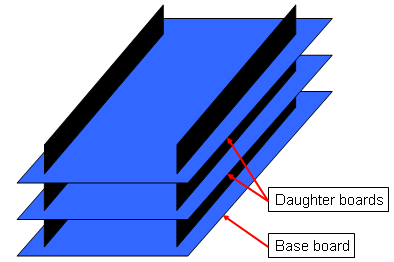
\includegraphics[width=0.75\textwidth, bb=0 0 394 262]{images/piggyback.png}
	\caption{Piggybacking of FLEX Boards}
	\label{fig:piggyback}
\end{figure}

\noindent As depicted in the Figure ~\ref{fig:piggyback}, several Daughter Boards, refer Section ~\ref{sec:daughter}, can be connected in piggyback fashion to the FLEX Base Board, refer Section ~\ref{sec:base}. The Daughter Boards have different features and they can be easily combined to obtain complex devices, refer Section ~\ref{sec:packs}. Evidence Srl and Embedded Solutions supply a growing number of Daughter Boards for basic and advanced applications.\\
%-----------------------------------------------------------------
\section{Base Boards}
\label{sec:base}
%-----------------------------------------------------------------
The FLEX Base Boards are designed to export all the connections of a standard Microchip dsPIC� DSC micro-controller. The board connections use the standard 2.54mm pitch; this feature make it easy the usage of customised (by Evidence) or home-made Daughter Boards.\\

\noindent The dsPIC� DSC micro-controllers can be mounted on boards in two different ways:
\begin{enumerate}
  \item by soldering the micro-controller directly on the surface of the board, or
  \item by  using a socket for installing the micro-controller through the interchangeable Plug-In Modules (PIMs) available from Microchip.
\end{enumerate}
With the later, the developer need not worry about the number of programming cycles during the implementation/test/debugging phases, as once the limit is reached, a new PIM can be installed on the socket replacing the older one.\\

\begin{figure}[!ht]
	\centering
		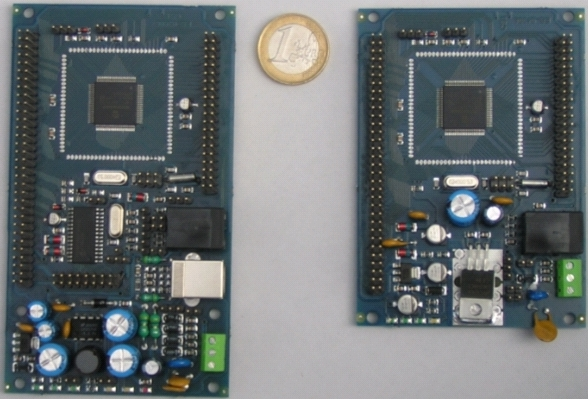
\includegraphics[width=0.90\textwidth,bb=0 0 588 399]{images/baseboards.jpg}
	\caption{FLEX Base Boards}
	\label{fig:base}
\end{figure}

\noindent As decipted in Figure ~\ref{fig:base}, The FLEX Base Board is available in two versions:
\begin{enumerate}
  \item Light version, refer Subsection ~\ref{subsec:001}
  \item Full version, refer Subsection ~\ref{subsec:003}
\end{enumerate}

\noindent The connectors of the Full and Light Versions are fully compatible, so that an application developed with the Full Version can be easily moved to the Light Version and vice-versa (i.e. with fewer or no modification to the control program).\\

\noindent Safety has been one of the most important aspect considered while engineering both versions of FLEX. Both the Base Boards are protected by a resettable fuse, permitting longer duration of the board, even when used by non-highly-skilled users (i.e. in school laboratories for students experiments).\\

\noindent Table ~\ref{tbl:base} compares FLEX Full with FLEX Light.
\begin{small}
\begin{table} [!ht]
\centering
\begin{tabular}{|p{0.8\columnwidth}|c|c|}
	\hline
	{\bf Features} & {\bf Full} & {\bf Light}\\
	\hline \hline
	Microchip dsPIC� DSC microcontroller dsPIC33FJ256MC710 & $\bullet$ & $\bullet$\\
  \hline
  Microchip PIC18� PIC18F2550 microcontroller for USB connection (programming using the USB port would be made available very soon) & $\bullet$ & \\
  \hline
  ICD2 in-circuit program connector & $\bullet$ & $\bullet$\\
  \hline
  USB connector for communication & $\bullet$ & \\
  \hline
  Set of LEDs for monitoring the board functioning status & $\bullet$ & $\bullet$\\
  \hline
  Set of connectors for Daughter boards piggybacking & $\bullet$ & $\bullet$\\
  \hline
  Power supply connectors & $\bullet$ & $\bullet$\\
  \hline
  Power supply circuitry with resettable fuses & $\bullet$ & $\bullet$\\
  \hline
  Simplified power supply (7 - 12V) & & $\bullet$\\
  \hline
  Extra-robust switching power supply (9 - 36V) & $\bullet$ & \\
  \hline
\end{tabular}
\caption{FLEX Full Vs FLEX Light}
\label{tbl:base}
\end{table}
\end{small}



%+-+-+-+-+-+-+-+-+-+-+-+-+-+-+-+-+-+-+-+-+-+-+-+-+-+-+-+-+-+-+-+-+
\clearpage
\subsection{[FLEX001] FLEX Light Base Board}
\label{subsec:001}
%+-+-+-+-+-+-+-+-+-+-+-+-+-+-+-+-+-+-+-+-+-+-+-+-+-+-+-+-+-+-+-+-+
The FLEX Light, as depicted in Figure ~\ref{fig:001}, has been designed to be as compact as possible. The Light Version uses a simplified power supply circuitry and there is no integrated USB programming capability. Target applications for the FLEX Light could be: distributed, battery-powered applications, like sensor networks; small robotic applications, i.e., for mobile robot control and sensor acquisition, etc.\\

\noindent The power supply of the FLEX Light varies in the range of 9 - 12V.\\

\begin{figure}[!ht]
	\centering
		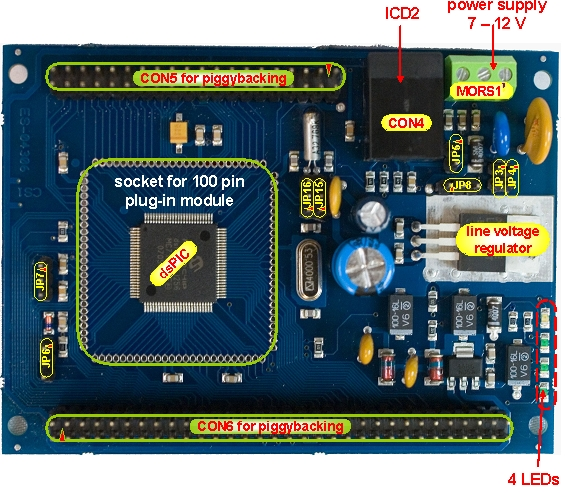
\includegraphics[width=0.90\textwidth,bb=0 0 582 493]{images/flex001.jpg}
	\caption{[FLEX001] FLEX Light Base Board}
	\label{fig:001}
\end{figure}

\noindent The main components of the FLEX Light are:
\begin {itemize}
  \item Microchip dsPIC� DSC microcontroller dsPIC33FJ256MC710
  \item A socket for the 100 pin Plug-In Module (PIM) available from Microchip
  \item An ICD2 programmer connector
  \item Power supply connectors
  \item A set of LEDs for monitoring the board functioning status
  \item Set of connectors for Daughter boards piggybacking
\end {itemize}


%^^^^^^^^^^^^^^^^^^^^^^^^^^^^^^^^^^^^^^^^^^^^^^^^^^
\subsubsection{Technical details}
\label{subsubsec:001tech}
%^^^^^^^^^^^^^^^^^^^^^^^^^^^^^^^^^^^^^^^^^^^^^^^^^^
\begin{figure}[!ht]
	\centering
		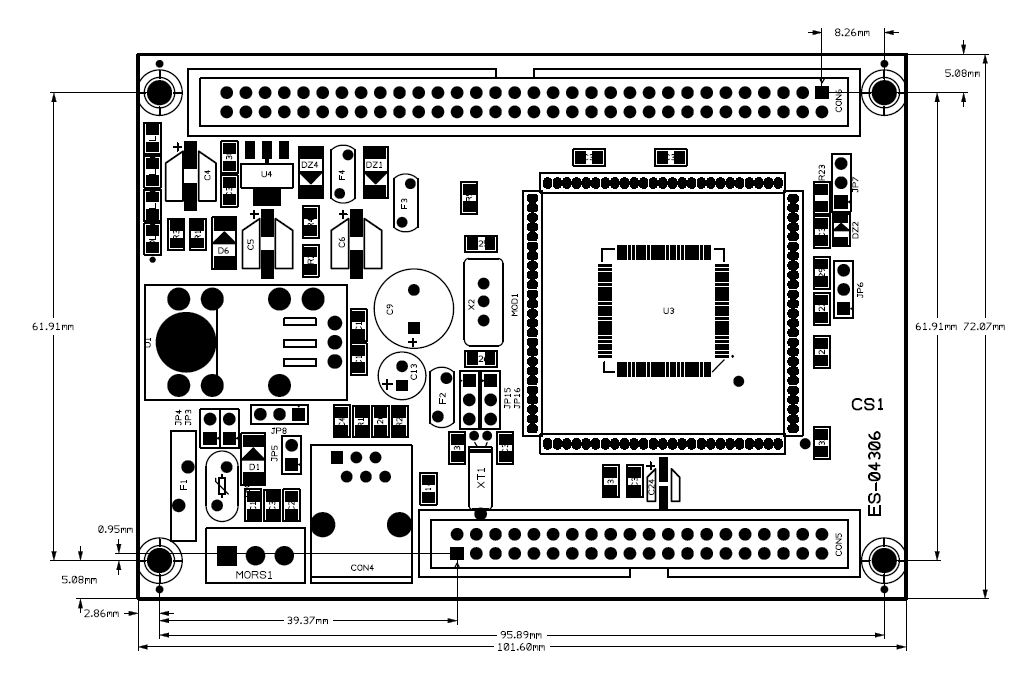
\includegraphics[width=0.90\textwidth,bb=0 0 1019 677]{images/001mec.png}
	\caption{[FLEX001] Dimensions of FLEX Light Base Board}
	\label{fig:001mec}
\end{figure}
\begin{figure}[!ht]
	\centering
		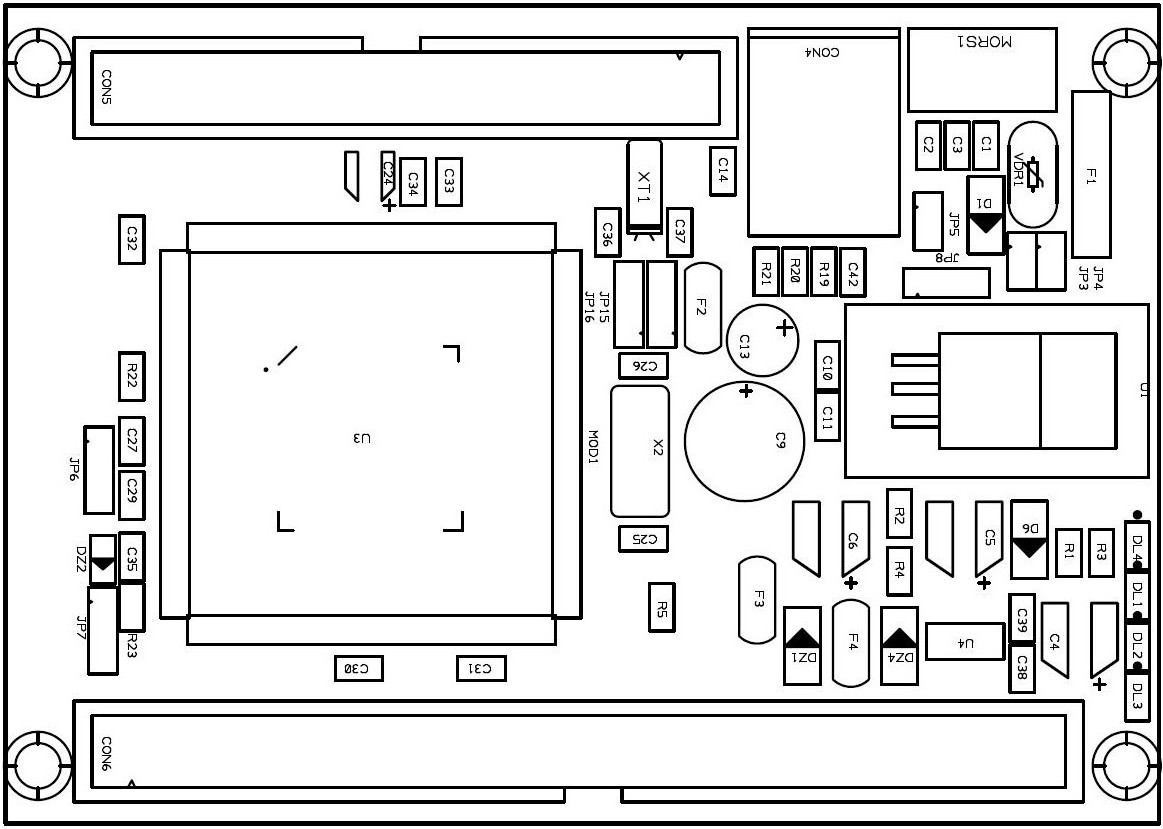
\includegraphics[width=0.90\textwidth,bb=0 0 1163 829]{images/001.png}
	\caption{[FLEX001] Details of FLEX Light Base Board}
	\label{fig:001detail}
\end{figure}


\begin{small}
\begin{table} [!ht]
\centering
\begin{tabular}{|c|l|}
  \hline
  Pin 1 & VIN\\
  \hline
  Pin 2 & GND\\
  \hline
  Pin 3 & EARTH\\
  \hline
\end{tabular}
\caption{FLEX001 - MORS1 (7-12 V power supply)}
\label{tbl:001mors1}
\end{table}
\end{small}


\begin{small}
\begin{table} [!ht]
\centering
\begin{tabular}{|l|l|}
  \hline
  DL1 (green) & Input power supply\\
  \hline
  DL2 (green) & Internal +5V power line activity\\
  \hline
  DL3 (green) & Internal +3V power line activity\\
  \hline
  DL4 (yellow) & dsPIC� DSC  (e.g. for debugging)\\
  \hline
\end{tabular}
\caption{FLEX001 - LEDs}
\label{tbl:001leds}
\end{table}
\end{small}


\begin{small}
\begin{table} [!ht]
\centering
\begin{tabular}{|c|c|c|}
  \hline
  {\bf Jumper} & {\bf pos. 1-2} & {\bf pos. 2-3}\\
  \hline
  JP3 & $\bullet$ GND & -\\
  \hline
  JP4 & $\bullet$ GND & -\\
  \hline
  JP5 & $\bullet$ EARTH & -\\
  \hline
  JP6 & $\bullet$ +3.3V & +AV DD$_{ext}$\\
  \hline
  JP7 & $\bullet$ GND & AV SS$_{ext}$\\
  \hline
  JP8 & +5V & $\bullet$ +3.3V\\
  \hline
  JP15 & SOSCI & $\bullet$ CRYSTAL\\
  \hline
  JP16 & SOSCO & $\bullet$ CRYSTAL\\
  \hline
  \multicolumn{3}{l}{\begin{tiny}Note: Default jumper settings are indicated by a $\bullet$\end{tiny}}\\
\end{tabular}
\caption{FLEX001 - Jumpers}
\label{tbl:001jps}
\end{table}
\end{small}


\begin{small}
\begin{table} [!ht]
\centering
\begin{tabular}{|l|l||l|l|}
  \hline
  Pin 1 & V$_{out}$ & Pin 2 & 5V$_{out}$\\
  \hline
  Pin 3 & Gnd$_{out}$ & Pin 4 & 3V$_{out}$\\
  \hline
  Pin 5 & INT3/RA14 & Pin 6 & GND\\
  \hline
  Pin 7 & IC1/RD8 & Pin 8 & INT4/RA15\\
  \hline
  Pin 9 & IC3/RD10 & Pin 10 & IC2/RD9\\
  \hline
  Pin 11 & OC1/RD0 & Pin 12 & IC4/RD11\\
  \hline
  Pin 13 & OC3/RD2 & Pin 14 & OC2/RD1\\
  \hline
  Pin 15 & IC5/RD12 & Pin 16 & OC4/RD3\\
  \hline
  Pin 17 & OC5/CN13/RD4 & Pin 18 & IC6/CN19/RD13\\
  \hline
  Pin 19 & OC7/CN15/RD6 & Pin 20 & OC6/CN14/RD5\\
  \hline
  Pin 21 & C1RX/RF0 & Pin 22 & OC8/UPDNCN16/RD7\\
  \hline
  Pin 23 & C2TX/RG1 & Pin 24 & C1TX/RF1\\
  \hline
  Pin 25 & AN22/CN22/RA6 & Pin 26 & C2RX/RG0\\
  \hline
  Pin 27 & PWM1L/RE0 & Pin 28 & AN23/CN23/RA7\\
  \hline
  Pin 29 & CSCK/RG14 & Pin 30 & PWM1H/RE1\\
  \hline
  Pin 31 & CSD0/RG13 & Pin 32 & CSDI/RG12\\
  \hline
  Pin 33 & PWM2H/RE3 & Pin 34 & PWM2L/RE2\\
  \hline
  Pin 35 & COFS/RG15 & Pin 36 & PWM3L/RE4\\
  \hline
  Pin 37 & PWM4L/RE6 & Pin 38 & PWM3H/RE5\\
  \hline
  Pin 39 & AN16/T2CK/T7CK/RC1 & Pin 40 & PWM4H/RE7\\
  \hline
\end{tabular}
\caption{FLEX001/FLEX003 - CON5 for Piggybacking}
\label{tbl:con5}
\end{table}
\end{small}


\begin{small}
\begin{table} [!ht]
\centering
\begin{tabular}{|l|l||l|l|}
  \hline
  Pin 1 & GND & Pin 2 & GND\\
  \hline
  Pin 3 & GND & Pin 4 & GND\\
  \hline
  Pin 5 & \begin{tiny}PGD2/EMUD2/SOSCI/CN1/RC13\end{tiny} & Pin 6 & \begin{tiny}PGC2/EMUC2/SOSCO/T1CK/CN0/RC14\end{tiny}\\
  \hline
  Pin 7 & AN17/T3CK/T6CK/RC2 & Pin 8 & AN18/T4CK/T9CK/RC3\\
  \hline
  Pin 9 & AN19/T5CK/T8CK/RC4 & Pin 10 & SCK2/CN8/RG6\\
  \hline
  Pin 11 & SDI2/CN9/RG7 & Pin 12 & SDO2/CN10/RG8\\
  \hline
  Pin 13 & DSP$_{MCLR}$ & Pin 14 & SS2/CN11/RG9\\
  \hline
  Pin 15 & TMS/RA0 & Pin 16 & AN20/FLTA/INT1/RE8\\
  \hline
  Pin 17 & AN21/FLTB/INT2/RE9 & Pin 18 & AN5/QEB/CN7/CN7/RB5\\
  \hline
  Pin 19 & AN4/QEA/CN6/RB4 & Pin 20 & AN3/INDX/CN5/RB3\\
  \hline
  Pin 21 & AN2/SS1/CN4/RB2 & Pin 22 & V$_{ref-}$/RA9\\
  \hline
  Pin 23 & V$_{ref+}$/RA10 & Pin 24 & AV DD$_{ext}$\\
  \hline
  Pin 25 & AV SS$_{ext}$ & Pin 26 & AN8/RB8\\
  \hline
  Pin 27 & AN9/RB9 & Pin 28 & AN10/RB10\\
  \hline
  Pin 29 & AN11/RB11 & Pin 30 & TCK/RA1\\
  \hline
  Pin 31 & U2CTS/RF12 & Pin 32 & U2RTS/RF13\\
  \hline
  Pin 33 & AN13/RB13 & Pin 34 & AN12/RB12\\
  \hline
  Pin 35 & IC7/U1CTS/CN20/RD14 & Pin 36 & AN15/OCFB/CN12/RB15\\
  \hline
  Pin 37 & U2RX/CN17/RF4 & Pin 38 & IC8/U1RTS/CN21/RD15\\
  \hline
  Pin 39 & U1TX/RF3 & Pin 40 & U2TX/CN18/RF5\\
  \hline
  Pin 41 & SDO1/RF8 & Pin 42 & U1RX/RF2\\
  \hline
  Pin 43 & SCK1/INT0/RF6 & Pin 44 & SDI1/RF7\\
  \hline
  Pin 45 & SCL1/RG2 & Pin 46 & SDA1/RG3\\
  \hline
  Pin 47 & SDA2/RA3 & Pin 48 & SCL2/RA2\\
  \hline
  Pin 49 & TD0/RA5 & Pin 50 & TDI/RA4\\
  \hline
  Pin 51 & PGD3/EMUD3/AN0/CN2/RB0 & Pin 52 & DSP$_{PCLK}$\\
  \hline
  Pin 53 & PGC3/EMUC3/AN1/CN3/RB1 & Pin 54 & DSP$_{PDATA}$\\
  \hline
  Pin 55 & 5V$_{out}$ & Pin 56 & 5V$_{out}$\\
  \hline
  Pin 57 & 3V$_{out}$ & Pin 58 & 3V$_{out}$\\
  \hline
  Pin 59 & GND & Pin 60 & GND\\
  \hline
  Pin 61 & V$_{out}$ & Pin 62 & V$_{out}$\\
  \hline
  Pin 63 & GND$_{out}$ & Pin 64 & GND$_{out}$\\
  \hline
\end{tabular}
\caption{FLEX001/FLEX003 - CON6 for Piggybacking}
\label{tbl:con6}
\end{table}
\end{small}



\begin{small}
\begin{table} [!ht]
\centering
\begin{tabular}{|l|}
  \hline
  $\bullet$ \hspace{0.1cm} {\tt CON4:} ICD2 connector\\
  \hline
\end{tabular}
\caption{FLEX001 - Other Connectors}
\label{tbl:001other}
\end{table}
\end{small}





%+-+-+-+-+-+-+-+-+-+-+-+-+-+-+-+-+-+-+-+-+-+-+-+-+-+-+-+-+-+-+-+-+
\clearpage
\subsection{[FLEX003] FLEX Full Base Board}
\label{subsec:003}
%+-+-+-+-+-+-+-+-+-+-+-+-+-+-+-+-+-+-+-+-+-+-+-+-+-+-+-+-+-+-+-+-+
The FLEX Full, as depicted in Figure ~\ref{fig:003}, integrates an extra-robust power supply circuitry, that allows usage of a wide range of power suppliers. It accepts voltage ranges between 9 - 36 volts. The power supply signal is filtered and adapted to the internal levels.\\
\begin{figure}[!ht]
	\centering
		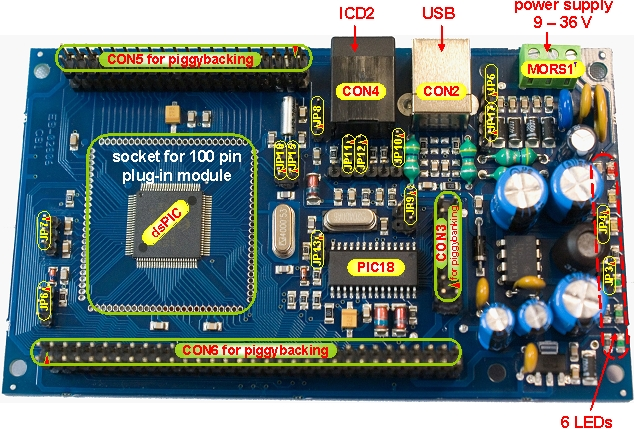
\includegraphics[width=0.90\textwidth,bb=0 0 635 436]{images/flex003.jpg}
	\caption{[FLEX003] FLEX Full Base Board}
	\label{fig:003}
\end{figure}

\noindent The FLEX Full also includes a native USB port which can be used for data transfer and, much more importantly as a programming interface for the onboard dsPIC� DSC. This option allows to save the cost of the ICD2 programming device, thereby making the development board fully self-contained.\\

\noindent {\tt Please note that the programming and debugging functionality on the PIC18 is not yet available. An application note will be available soon with all the needed information on how to implement the programmer functionality on the PIC18. The debugger functionality will be available as special version of the FLEX Full.}\\
 
\noindent The main components of FLEX Full are: 
\begin {itemize}
  \item Microchip dsPIC� DSC microcontroller dsPIC33FJ256MC710
  \item A socket for the 100 pin Plug-In Module (PIM) available from Microchip
  \item An ICD2 programmer connector
  \item A USB connector for direct programming
  \item Power supply connectors
  \item A set of LEDs for monitoring the board functioning status
  \item An onboard Microchip PIC18� PIC18F2550 microcontroller for integrated programming
  \item Set of connectors for Daughter boards piggybacking
\end {itemize}


%^^^^^^^^^^^^^^^^^^^^^^^^^^^^^^^^^^^^^^^^^^^^^^^^^^
\subsubsection{Technical details}
\label{subsubsec:003tech}
%^^^^^^^^^^^^^^^^^^^^^^^^^^^^^^^^^^^^^^^^^^^^^^^^^^
\begin{figure}[!ht]
	\centering
		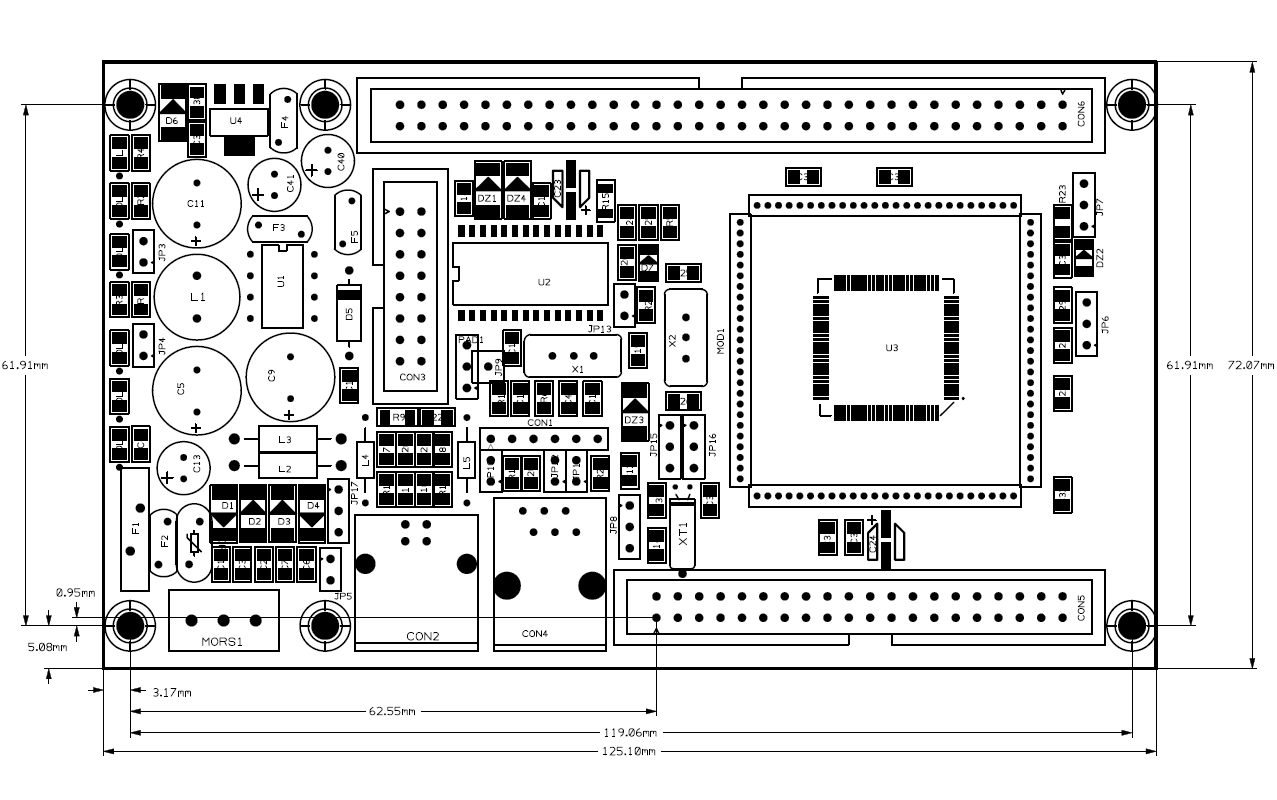
\includegraphics[width=0.90\textwidth,bb=0 0 1277 800]{images/003mec.png}
	\caption{[FLEX003] Dimensions of FLEX Full Base Board}
	\label{fig:003mec}
\end{figure}
\begin{figure}[!ht]
	\centering
		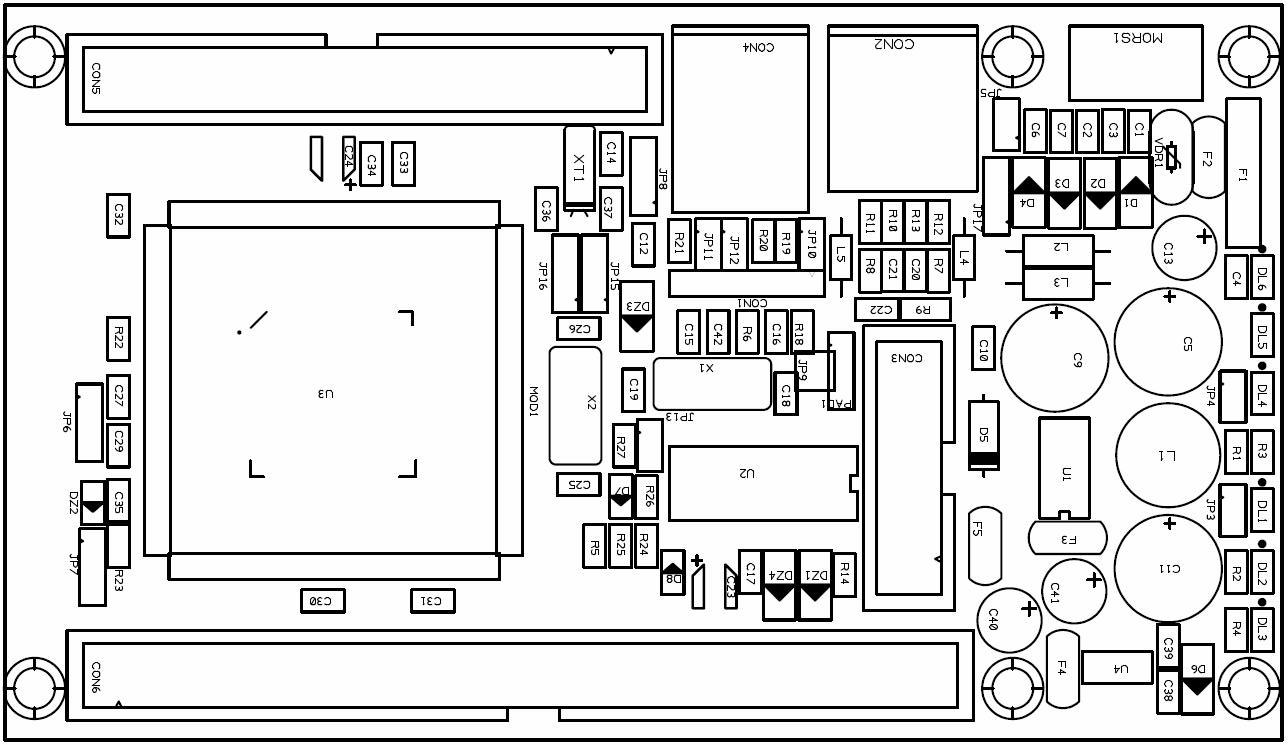
\includegraphics[width=0.90\textwidth,bb=0 0 1288 745]{images/003.png}
	\caption{[FLEX003] Details of FLEX Full Base Board}
	\label{fig:003detail}
\end{figure}

\begin{small}
\begin{table} [!ht]
\centering
\begin{tabular}{|c|l|}
  \hline
  Pin 1 & VINA\\
  \hline
  Pin 2 & VINB\\
  \hline
  Pin 3 & EARTH\\
  \hline
\end{tabular}
\caption{FLEX003 - MORS1 (9-36 V power supply)}
\label{tbl:003mors1}
\end{table}
\end{small}


\begin{small}
\begin{table} [!ht]
\centering
\begin{tabular}{|l|l|}
  \hline
  DL1 (green) & Input power supply\\
  \hline
  DL2 (green) & Internal +5V power line activity\\
  \hline
  DL3 (green) & Internal +3V power line activity\\
  \hline
  DL4 (yellow) & dsPIC� DSC  (e.g. for debugging)\\
  \hline
  DL5 (yellow) & Internal PIC18\\
  \hline
  DL6 (red) & USB cable connection monitor\\
  \hline
\end{tabular}
\caption{FLEX003 - LEDs}
\label{tbl:003leds}
\end{table}
\end{small}


\begin{small}
\begin{table} [!ht]
\centering
\begin{tabular}{|c|c|c|}
  \hline
  {\bf Jumper} & {\bf pos. 1-2} & {\bf pos. 2-3}\\
  \hline
  JP3 & $\bullet$ GND & -\\
  \hline
  JP4 & $\bullet$ GND & -\\
  \hline
  JP5 & $\bullet$ EARTH & -\\
  \hline
  JP6 & $\bullet$ +3.3V & +AV DD$_{ext}$\\
  \hline
  JP7 & $\bullet$ GND & AV SS$_{ext}$\\
  \hline
  JP8 & +5V & $\bullet$ +3.3V\\
  \hline
  JP9 & +USB & $\bullet$ +5V\\
  \hline
  JP10 & $\bullet$ DSP\_MCLR & PIC18\_MCLR\\
  \hline
  JP11 & $\bullet$ DSP\_PDATA & PIC18\_PDATA\\
  \hline
  JP12 & $\bullet$ DSP\_PCLK & PIC18\_PCLK\\
  \hline
  JP13 & VDD pull up & -\\
  \hline
  JP15 & SOSCI & $\bullet$ CRYSTAL\\
  \hline
  JP16 & SOSCO & $\bullet$ CRYSTAL\\
  \hline
  JP17 & $\bullet$ GND & EARTH\\
  \hline
  \multicolumn{3}{l}{\begin{tiny}Note: Default jumper settings are indicated by a $\bullet$\end{tiny}}\\
\end{tabular}
\caption{FLEX003 - Jumpers}
\label{tbl:003jps}
\end{table}
\end{small}


\begin{small}
\begin{table} [!ht]
\centering
\begin{tabular}{|l|l||l|l|}
  \hline
  Pin 1 & +VDD$_{out}$ & Pin 2 & GND\\
  \hline
  Pin 3 & RA0/AN0 & Pin 4 & RB4/AN11/KB10\\
  \hline
  Pin 5 & RA1/AN1 & Pin 6 & RB3/AN9/CCP2/VPO\\
  \hline
  Pin 7 & RA2/AN2/V$_{ref-}$/CV$_{ref}$ & Pin 8 & RC7/RX/DT/SDO\\
  \hline
  Pin 9 & RA3/AN3/Vref+ & Pin 10 & RC6/TX/CK\\
  \hline
  Pin 11 & RA5/AN4/HLVDin/C2$_{out}$ & Pin 12 & RC2/CCP1\\
  \hline
  Pin 13 & RC1/T1OSI/CCP2/UOE\# & Pin 14 & RA4/T0CKI/C1$_{out}$/RCV\\
  \hline
  Pin 15 & L$_{MCLR}$ & Pin 16 & RC0/T1OSO/T1CKI\\
  \hline
\end{tabular}
\caption{FLEX003 - CON3 for Piggybacking (PIC18F2550)}
\label{tbl:con3}
\end{table}
\end{small}


\begin{small}
\begin{table} [!ht]
\centering
\begin{tabular}{|l|}
  \hline
  $\bullet$ \hspace{0.1cm} {\tt CON2:} USB connector\\
  $\bullet$ \hspace{0.1cm} {\tt CON4:} ICD2 connector\\
  $\bullet$ \hspace{0.1cm} {\tt CON5:} 40 pin piggybacking connector, refer Table \ref{tbl:con5} \\
  $\bullet$ \hspace{0.1cm} {\tt CON6:} 64 pin piggybacking connector, refer Table \ref{tbl:con6} \\
  \hline
\end{tabular}
\caption{FLEX003 - Other Connectors}
\label{tbl:003other}
\end{table}
\end{small}


\begin{small}
\begin{table} [!ht]
\centering
\begin{tabular}{|c|c|c|}
  \hline
  {\bf Jumper} & {\bf pos. 1-2} & {\bf pos. 2-3}\\
  \hline
  JP3 & $\bullet$ & -\\
  \hline
  JP4 & $\bullet$ & -\\
  \hline
  JP5 & $\bullet$ & -\\
  \hline
  JP6 & $\bullet$ & \\
  \hline
  JP7 & $\bullet$ & \\
  \hline
  JP8 & $\bullet$ & \\
  \hline
  JP9 &  & $\bullet$\\
  \hline
  JP10 &  & $\bullet$\\
  \hline
  JP11 &  & $\bullet$\\
  \hline
  JP12 &  & $\bullet$\\
  \hline
  JP13 &  & -\\
  \hline
  JP15 &  & $\bullet$\\
  \hline
  JP16 &  & $\bullet$\\
  \hline
  JP17 & $\bullet$ & \\
  \hline
\end{tabular}
\caption{FLEX003 - Jumper settings for programming PIC18}
\label{tbl:003pic18}
\end{table}
\end{small}
%-----------------------------------------------------------------
\section{Daughter boards}
\label{sec:daughter}
%-----------------------------------------------------------------
A FLEX Daughter Board is a board with specialized features that can be added on top of a FLEX Base Board, refer Section  ~\ref{sec:base} (by piggybacking, refer Figure ~\ref{fig:piggyback}), to obtain complex devices for all possible applications.\\

\noindent Evidence Srl and Embedded Solutions propose a set of general purpose Daughter Boards for some of the most common applications.\\

\noindent The development of customised, refer Section ~\ref{sec:custom}, or home-made Daughter Boards are made easy as the FLEX Base Board connectors uses the standard 2.54mm pitch. Hence, virtually, the extending of features of the FLEX platform, refer Table ~\ref{tbl:base}, is unlimited.



%+-+-+-+-+-+-+-+-+-+-+-+-+-+-+-+-+-+-+-+-+-+-+-+-+-+-+-+-+-+-+-+-+
\subsection{[FLEX100] FLEX Thru Hole Daughter Board}
\label{subsec:100}
%+-+-+-+-+-+-+-+-+-+-+-+-+-+-+-+-+-+-+-+-+-+-+-+-+-+-+-+-+-+-+-+-+
The board, depicted in Figure ~\ref{fig:100}, is targeted for the development of small, homemade, custom circuits that can be transparently interfaced with the FLEX Base Boards, refer Figure ~\ref{fig:base}.\\

\begin{figure}[!ht]
	\centering
		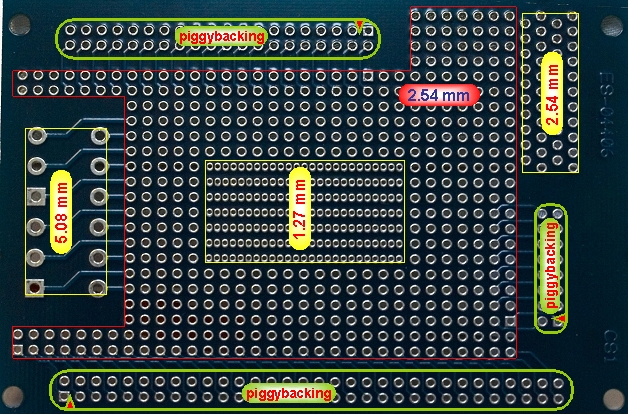
\includegraphics[width=0.90\textwidth,bb=0 0 629 415]{images/flex100.jpg}
	\caption{[FLEX100] FLEX Thru Hole Daughter Board}
	\label{fig:100}
\end{figure}

\noindent The board makes available to the user several common pinholes for connecting electronic components. Pinholes marked with "piggybacking" are pins which come from the piggybacked FLEX board, refer Figure ~\ref{fig:piggyback}, and each pin on the piggybacking row is connected to a pin on the most wide board section.\\


%^^^^^^^^^^^^^^^^^^^^^^^^^^^^^^^^^^^^^^^^^^^^^^^^^^
\subsubsection{Technical details}
\label{subsubsec:100tech}
%^^^^^^^^^^^^^^^^^^^^^^^^^^^^^^^^^^^^^^^^^^^^^^^^^^
\begin{small}
\begin{table}[!ht]
\centering
\begin{tabular}{|l|}
  \hline
  $\bullet$ \hspace{0.1cm} {\tt CON3:} 16 pin connector, refer Table ~\ref{tbl:con3}\\
  $\bullet$ \hspace{0.1cm} {\tt CON5:} 40 pin connector, refer Table ~\ref{tbl:con5}\\
  $\bullet$ \hspace{0.1cm} {\tt CON6:} 64 pin connector, refer Table ~\ref{tbl:con6}\\
  \hline
\end{tabular}
\caption{FLEX100 - Standard Connectors for Piggybacking}
\label{tbl:100piggy}
\end{table}
\end{small}

\begin{small}
\begin{table}[!ht]
\centering
\begin{tabular}{|l|}
  \hline
  $\bullet$ \hspace{0.1cm} 5.08 mm for clamps\\
  $\bullet$ \hspace{0.1cm} 2.54 mm for RJ45, RS232, etc. connectors\\
  $\bullet$ \hspace{0.1cm} 2.54 mm for all other components\\
  $\bullet$ \hspace{0.1cm} 1.27 mm for typical SMD components\\
  \hline
\end{tabular}
\caption{FLEX100 - Standard Pinhole Patterns}
\label{tbl:100pattern}
\end{table}
\end{small}



%+-+-+-+-+-+-+-+-+-+-+-+-+-+-+-+-+-+-+-+-+-+-+-+-+-+-+-+-+-+-+-+-+
\clearpage
\subsection{[FLEX101] FLEX Multibus Base Daughter Board}
\label{subsec:101}
%+-+-+-+-+-+-+-+-+-+-+-+-+-+-+-+-+-+-+-+-+-+-+-+-+-+-+-+-+-+-+-+-+
The FLEX Multibus Base Board, as depicted in Figure ~\ref{fig:101}, is a FLEX Daughter Board, refer Section ~\ref{sec:daughter}. It fits directly on FLEX Base Board (FLEX Full, refer Subsection ~\ref{subsec:001}/FLEX Light, refer Subsection ~\ref{subsec:003}), and number of slots, refer Table ~\ref{tbl:101slots}, are available for FLEX Multibus Modules to be mounted on top of it, thereby extending the FLEX platform.\\

\begin{figure}[!ht]
	\centering
		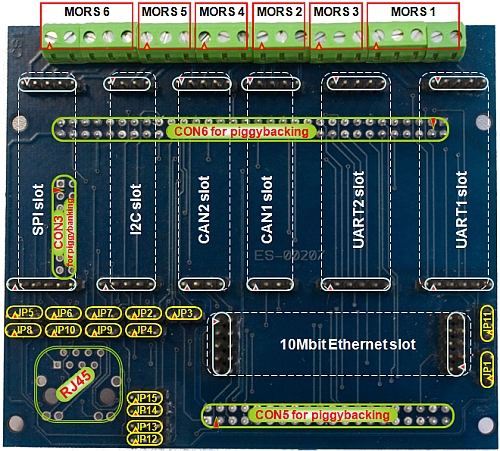
\includegraphics[width=0.90\textwidth,bb=0 0 541 500]{images/flex101.jpg}
	\caption{[FLEX101] FLEX Multibus Base Daughter Board}
	\label{fig:101}
\end{figure}
\noindent {\tt Note: The RJ45 Ethernet Connecter is not included with this product. It is sold along with the FLEX Multibus Ethernet Module, refer Subsection ~\ref{subsec:102}, and has to be soldered on the FLEX Multibus Base Daughter Board}.\\

\noindent The following slots are available on the Multibus board:
\begin{itemize}
  \item UART2 slot, for Serial TTL/RS232/RS485/RS422 module
  \item UART1 slot, for Serial TTL/RS232/RS485 module
  \item CAN1 slot, for CAN module
  \item CAN2 slot, for CAN module
  \item I2C slot (channel selectable), for I2C module
  \item SPI slot (channel selectable), for SPI module
  \item Ethernet slot, for 10Mbit Ethernet module
\end{itemize}
\noindent {\tt Note: Modules are mounted only if needed. For example, if the application requires the Ethernet interface and the connection to the CAN bus, only the corresponding modules will be mounted on the Multibus Base Board, leaving the remaining pins free for other use}.\\

\noindent {\bf Chip select of SPI Module (Slot 6):} Jumpers JP8, JP9, and JP10 control the chip select of the SPI module from either a general purpose I/O or chip select pin built-in in the microcontroller, refer Figures ~\ref{fig:101detail} and ~\ref{fig:101slot6} and Tables ~\ref{tbl:101jps} and ~\ref{tbl:107slot6_jps}.\\



%^^^^^^^^^^^^^^^^^^^^^^^^^^^^^^^^^^^^^^^^^^^^^^^^^^
\subsubsection{Technical details}
\label{subsubsec:101tech}
%^^^^^^^^^^^^^^^^^^^^^^^^^^^^^^^^^^^^^^^^^^^^^^^^^^
\begin{figure}[!ht]
	\centering
		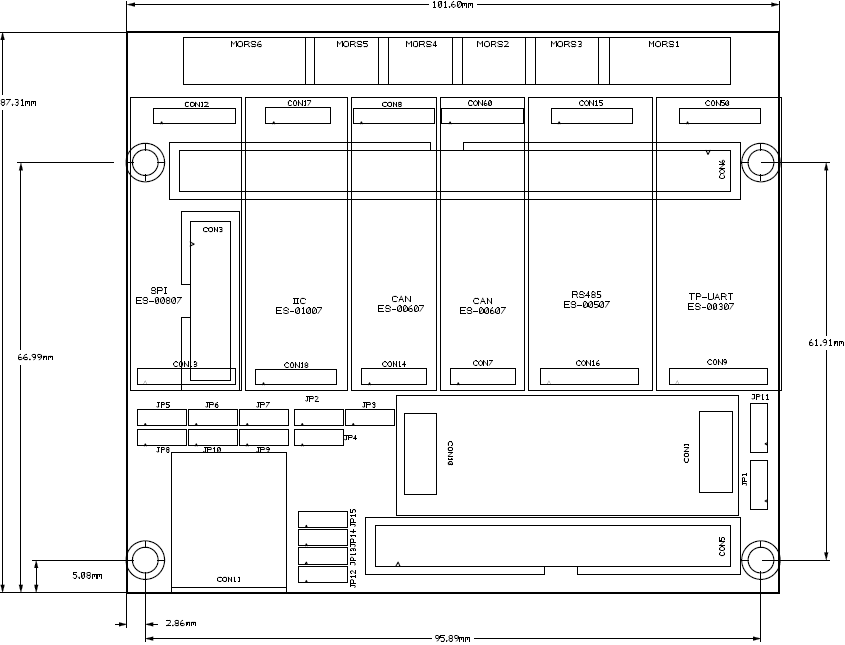
\includegraphics[width=0.90\textwidth,bb=0 0 845 645]{images/101mec.png}
	\caption{[FLEX101] Dimensions of FLEX Multibus Base Daughter Board}
	\label{fig:101mec}
\end{figure}
\begin{figure}[!ht]
	\centering
		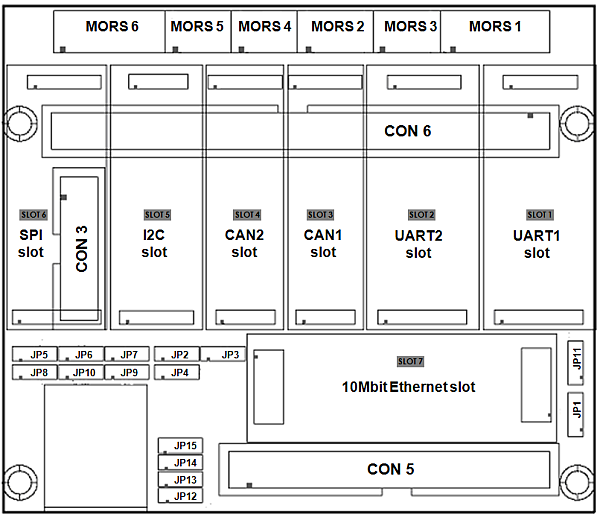
\includegraphics[width=0.90\textwidth,bb=0 0 662 589]{images/101.png}
	\caption{[FLEX101] Details of FLEX Multibus Base Daughter Board}
	\label{fig:101detail}
\end{figure}

\begin{small}
\begin{table}[!ht]
\centering
\begin{tabular}{|c|l|}
	\hline
	Pin 1 & CTS PC\\
  \hline
	Pin 2 & RX PC\\
	\hline
  Pin 3 & TX PC\\
	\hline
  Pin 4 & RTS PC\\
	\hline
  Pin 5 & GND \\
	\hline
\end{tabular}
\caption{FLEX101 - MORS1 (RS232 module)}
\label{tbl:101mors1}
\end{table}
\end{small}

\begin{small}
\begin{table}[!ht]
\centering
\begin{tabular}{|c|l|}
	\hline
	Pin 1 & O\_CAN+\\
	\hline
  Pin 2 & O\_CAN-\\
	\hline
  Pin 3 & GND\\
	\hline
\end{tabular}
\caption{FLEX101 - MORS2 (CAN1 module)}
\label{tbl:101mors2}
\end{table}
\end{small}

\begin{small}
\begin{table}[!ht]
\centering
\begin{tabular}{|c|l|}
	\hline
	Pin 1 & 485-\\
	\hline
  Pin 2 & 485+\\
	\hline
  Pin 3 & GND\\
	\hline
\end{tabular}
\caption{FLEX101 - MORS3 (RS485 module)}
\label{tbl:101mors3}
\end{table}
\end{small}

\begin{small}
\begin{table}[!ht]
\centering
\begin{tabular}{|c|l|}
	\hline
	Pin 1 & O\_CAN+1\\
	\hline
  Pin 2 & O\_CAN-1\\
	\hline
  Pin 3 & GND \\
	\hline
\end{tabular}
\caption{FLEX101 - MORS4 (CAN2 module)}
\label{tbl:101mors4}
\end{table}
\end{small}

\begin{small}
\begin{table}[!ht]
\centering
\begin{tabular}{|c|l|}
	\hline
	Pin 1 & IIC\_DIO\_C\\
	\hline
  Pin 2 & IIC\_CK\_C\\
	\hline
  Pin 3 & GND \\
	\hline
\end{tabular}
\caption{FLEX101 - MORS5 (I2C module)}
\label{tbl:101mors5}
\end{table}
\end{small}

\begin{small}
\begin{table}[!ht]
\centering
\begin{tabular}{|c|l|}
	\hline
	Pin 1 & SPI\_DO\_C\\
	\hline
  Pin 2 & SPI\_DI\_C\\
	\hline
  Pin 3 & SPI\_CLK\_C\\
	\hline
  Pin 4 & SPI\_SS\_C\\
  \hline
  Pin 5 & GND\\
	\hline
\end{tabular}
\caption{FLEX101 - MORS6 (SPI module)}
\label{tbl:101mors6}
\end{table}
\end{small}

\begin{small}
\begin{table}[!ht]
\centering
\begin{tabular}{|c|c|c|}
  \hline
  {\bf Jumper} & {\bf pos. 1-2} & {\bf pos. 2-3}\\
  \hline
	JP1 & FRCK\_1 & RESN \\
  \hline
	JP2 & IIC\_2 DIO & IIC\_1 DIO\\
	\hline
  JP3 & IIC\_2 CLK & IIC\_1 CLK\\
	\hline
  JP4 & IIC\_2 CS & IIC\_1 CS\\
	\hline
  JP5 & SPI\_2 DI & SPI\_1 DI\\
	\hline
  JP6 & SPI\_2 DO & SPI\_1 DO\\
	\hline
  JP7 & SPI\_2 CLK & SPI\_1 CLK\\
	\hline
  JP8 & SPI\_1 SS\_up & SPI\_1 SS\\
	\hline
  JP9 & SPI\_2 SS JP8/JP10 & SPI\_1 SS JP8/JP9\\
	\hline
  JP10 & SPI\_2 SS\_up & SPI\_2 SS\\
	\hline
  JP11 & GND & GND\_OUT\\
	\hline
  JP12 & LAN SPI\_2 DI & LAN SPI\_1 DI\\
	\hline
  JP13 & LAN SPI\_2 DO & LAN SPI\_1 DO\\
	\hline
  JP14 & LAN SPI\_2 CLK & LAN SPI\_1 CLK\\
	\hline
  JP15 & LAN SPI\_2 SS & LAN SPI\_1 SS\\
	\hline
  \multicolumn{3}{l}{\begin{tiny}Note: Default jumper settings are indicated by a $\bullet$\end{tiny}}\\
\end{tabular}
\caption{FLEX101 - Jumpers}
\label{tbl:101jps}
\end{table}
\end{small}

\begin{small}
\begin{table}[!ht]
\centering
\begin{tabular}{|l|}
  \hline
  $\bullet$ \hspace{0.1cm} {\tt CON3:} 16 pin piggybacking connector, refer Table ~\ref{tbl:con3} \\
  $\bullet$ \hspace{0.1cm} {\tt CON5:} 40 pin piggybacking connector, refer Table ~\ref{tbl:con5} \\
  $\bullet$ \hspace{0.1cm} {\tt CON6:} 64 pin piggybacking connector, refer Table ~\ref{tbl:con6} \\
  \hline
\end{tabular}
\caption{FLEX101 - Other Connectors}
\label{tbl:101other}
\end{table}
\end{small}


\begin{small}
\begin{table}[!ht]
\centering
\begin{tabular}{|c|c|c|c|c|c|c|}
	\hline
	{\bf Module} & {\bf Slot1} & {\bf Slot2} & {\bf Slot3} & {\bf Slot4} & {\bf Slot5} & {\bf Slot6}\\
	\hline
	RS232 (FLEX103) & $\bullet$ & $\bullet$ &  &  &  & \\
	\hline
  RS485 (FLEX104) & $\bullet$ & $\bullet$ &  &  &  & \\
	\hline
  RS422 (FLEX105) & $\bullet$ &  &  &  &  & \\
	\hline
  CAN (FLEX106) &  &  & $\bullet$ & $\bullet$ &  & \\
	\hline
  SPI (FLEX107) &  &  &  &  &  & $\bullet$ \\
	\hline
  Serial TTL (FLEX108) & $\bullet$ & $\bullet$ &  &  &  & \\
	\hline
  I2C &  &  &  &  & $\bullet$ & \\
	\hline
\end{tabular}
\caption{FLEX101 - Slot Allocation}
\label{tbl:101slots}
\end{table}
\end{small}
%|||||||||||||||||||||||||||||||||||||||||||||||||||||||||
\begin{figure}[!ht]
	\centering
		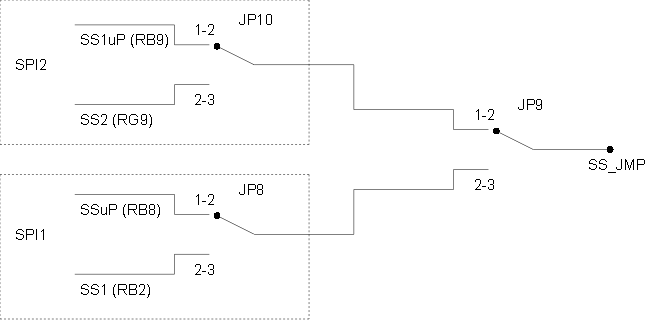
\includegraphics[width=0.50\textwidth,bb=0 0 648 320]{images/101slot6.png}
		%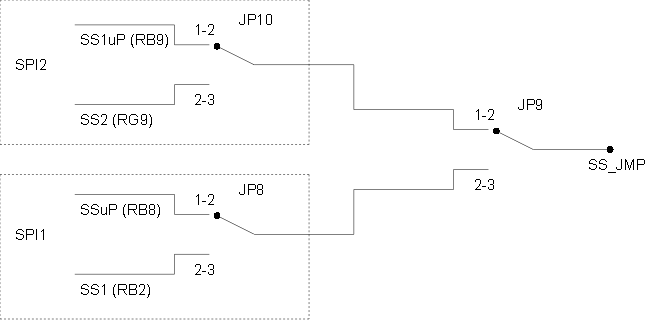
\includegraphics[width=0.50\textwidth]{images/101slot6.eps}
	\caption{[FLEX101] SPI Chip Select (Slot6) Jumper Settings}
	\label{fig:101slot6}
\end{figure}

\begin{small}
\begin{table}[!ht]
\centering
\begin{tabular}{|c|c|c|c|}
	\hline
	{\bf JP8} & {\bf JP9} & {\bf JP10} & {\bf Chip select from}\\
  \hline
   & 1-2 & 1-2 & RB9\\
	\hline
   & 1-2 & 2-3 & SS2 (RG9)\\
   \hline
  1-2 & 2-3 & & RB8\\
   \hline
  2-3 & 2-3 & & SS1 (RB2)\\
  \hline
\end{tabular}
\caption{FLEX101 - SPI Chip Select (Slot6) Jumper Settings}
\label{tbl:107slot6_jps}
\end{table}
\end{small}
%|||||||||||||||||||||||||||||||||||||||||||||||||||||||||
\clearpage
\noindent {\bf {\large Multibus Modules}}\\

\noindent The FLEX Multibus Modules are piggybacked on the FLEX Multibus Base Daughter Board, refer Subsection ~\ref{subsec:101}. These are the most widely used serial communication standards currently available: 

%+-+-+-+-+-+-+-+-+-+-+-+-+-+-+-+-+-+-+-+-+-+-+-+-+-+-+-+-+-+-+-+-+
\subsection{[FLEX102] FLEX Multibus Ethernet Module}
\label{subsec:102}
%+-+-+-+-+-+-+-+-+-+-+-+-+-+-+-+-+-+-+-+-+-+-+-+-+-+-+-+-+-+-+-+-+
The board, depicted in Figure ~\ref{fig:102}, is the Ethernet Module. It fits on slot 7 of the FLEX Multibus Base Daughter Board, refer Figure ~\ref{fig:101detail}.\\
\noindent The module can be used to export an ethernet connection through the RJ45 connector available on the Multibus Base Board. The ethernet chip used is the Microchip ENC28J60, which is connected to the dsPIC� by using the SPI bus.\\

\begin{figure}[!ht]
	\centering
		\includegraphics[width=0.50\textwidth,bb=0 0 500 200]{images/flex102.jpg}
	\caption{[FLEX102] FLEX Multibus Ethernet Module}
	\label{fig:102}
\end{figure}

\noindent {\tt Note: One RJ45 Ethernet Connecter is included with this product. It is to be soldered on the FLEX Multibus Base Daughter Board, refer Figure ~\ref{fig:101}.}\\

%^^^^^^^^^^^^^^^^^^^^^^^^^^^^^^^^^^^^^^^^^^^^^^^^^^
\subsubsection{Technical details}
\label{subsubsec:102tech}
%^^^^^^^^^^^^^^^^^^^^^^^^^^^^^^^^^^^^^^^^^^^^^^^^^^
\begin{figure}[!ht]
	\centering
		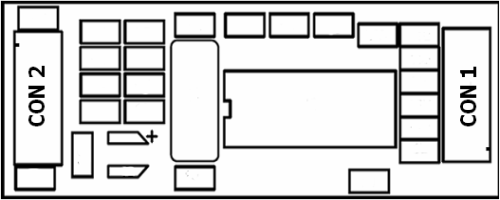
\includegraphics[width=0.50\textwidth,bb=0 0 500 200]{images/102.png}
	\caption{[FLEX102] Details of FLEX Multibus Ethernet Module}
	\label{fig:102detail}
\end{figure}

\begin{small}
\begin{table}[!ht]
\centering
\begin{tabular}{|l|l||l|l|}
	\hline
	Pin 1 & SDO\_2 & Pin 2 & SCK\_2\\
	\hline
	Pin 3 & SDI\_2 & Pin 4 & RE\_4\\
	\hline
	Pin 5 & SS\_2 & Pin 6 & INT\_4\\
	\hline
	Pin 7 & CN\_1 & Pin 8 & INT\_3\\
	\hline
	Pin 9 & GND & Pin 10 & +3.3V\\
	\hline
\end{tabular}
\caption{FLEX102 - CON1}
\label{tbl:102con1}
\end{table}
\end{small}

\begin{small}
\begin{table}[!ht]
\centering
\begin{tabular}{|l|l||l|l|}
	\hline
	Pin 1 & LED\_A & Pin 2 & TPOUT +3.3V\\
	\hline
  Pin 3 & TPOUT- & Pin 4 & TPOUT+\\
	\hline
  Pin 5 & - & Pin 6 & TPIN GND \\
	\hline
  Pin 7 & TPIN- & Pin 8 & TPIN+\\
	\hline
  Pin 9 & LED\_B & Pin 10 & GND\\
	\hline
\end{tabular}
\caption{FLEX102 - CON2}
\label{tbl:102con2}
\end{table}
\end{small}



%+-+-+-+-+-+-+-+-+-+-+-+-+-+-+-+-+-+-+-+-+-+-+-+-+-+-+-+-+-+-+-+-+
\clearpage
\subsection{[FLEX103] FLEX Multibus RS232 Module}
\label{subsec:103}
%+-+-+-+-+-+-+-+-+-+-+-+-+-+-+-+-+-+-+-+-+-+-+-+-+-+-+-+-+-+-+-+-+
The board, depicted in Figure ~\ref{fig:103}, is the Rs232 Module. It fits on slot 1 and/or slot 2 of the FLEX Multibus Base Daughter Board, refer Figure ~\ref{fig:101detail}.\\
\noindent This module can be used to export the UART pins linked to the UART peipherals on the dsPIC� by using signals which are compatible with the RS232 standard.\\

\begin{figure}[!ht]
	\centering
		\includegraphics[width=0.50\textwidth,bb=0 0 500 200]{images/flex103.jpg}
	\caption{[FLEX103] FLEX Multibus RS232 Module}
	\label{fig:103}
\end{figure}


%^^^^^^^^^^^^^^^^^^^^^^^^^^^^^^^^^^^^^^^^^^^^^^^^^^
\subsubsection{Technical details}
\label{subsubsec:103tech}
%^^^^^^^^^^^^^^^^^^^^^^^^^^^^^^^^^^^^^^^^^^^^^^^^^^
\begin{figure}[!ht]
	\centering
		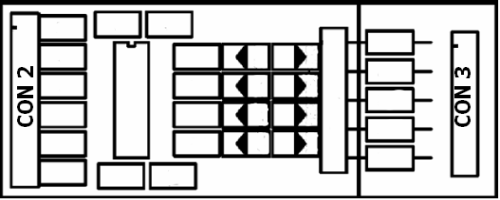
\includegraphics[width=0.50\textwidth,bb=0 0 500 200]{images/103.png}
	\caption{[FLEX103] Details of FLEX Multibus RS232 Module}
	\label{fig:103detail}
\end{figure}

\begin{small}
\begin{table}[!ht]
\centering
\begin{tabular}{|c|l|}
	\hline
	Pin 1 & +5V\\
	\hline
  Pin 2 & TX\_1\\
	\hline
  Pin 3 & SCK\_1\\
	\hline
  Pin 4 & RX\_1\\
	\hline
  Pin 5 & FRCK\_1\\
	\hline
  Pin 6 & GND\\
	\hline
\end{tabular}
\caption{FLEX103 - CON2}
\label{tbl:103con2}
\end{table}
\end{small}

\begin{small}
\begin{table}[!ht]
\centering
\begin{tabular}{|c|l|}
	\hline
	Pin 1 & CTS PC\\
	\hline
  Pin 2 & RX PC\\
	\hline
  Pin 3 & TX PC\\
	\hline
  Pin 4 & RTS PC\\
	\hline
  Pin 5 & GND\\
	\hline
\end{tabular}
\caption{FLEX103 - CON3}
\label{tbl:103con3}
\end{table}
\end{small}



%+-+-+-+-+-+-+-+-+-+-+-+-+-+-+-+-+-+-+-+-+-+-+-+-+-+-+-+-+-+-+-+-+
\clearpage
\subsection{[FLEX104] FLEX Multibus RS485 Module}
\label{subsec:104}
%+-+-+-+-+-+-+-+-+-+-+-+-+-+-+-+-+-+-+-+-+-+-+-+-+-+-+-+-+-+-+-+-+
The board, depicted in Figure ~\ref{fig:104}, is the RS485 Module. It fits on slot 1 and/or slot 2 of the FLEX Multibus Base Daughter Board, refer Figure ~\ref{fig:101detail}.\\
\noindent This module can be used to export the UART pins linked to the UART peipherals on the dsPIC� by using signals which are compatible with the RS485 standard.\\

\begin{figure}[!ht]
	\centering
		\includegraphics[width=0.50\textwidth,bb=0 0 500 200]{images/flex104.jpg}
	\caption{[FLEX104] FLEX Multibus RS485 Module}
	\label{fig:104}
\end{figure}


%^^^^^^^^^^^^^^^^^^^^^^^^^^^^^^^^^^^^^^^^^^^^^^^^^^
\subsubsection{Technical details}
\label{subsubsec:104tech}
%^^^^^^^^^^^^^^^^^^^^^^^^^^^^^^^^^^^^^^^^^^^^^^^^^^
\begin{figure}[!ht]
	\centering
		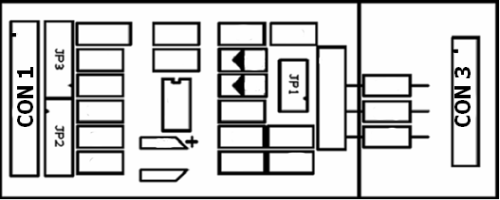
\includegraphics[width=0.50\textwidth,bb=0 0 500 200]{images/104.png}
	\caption{[FLEX104] Details of FLEX Multibus RS485 Module}
	\label{fig:104detail}
\end{figure}

\begin{small}
\begin{table} [h]
\centering
\begin{tabular}{|c|c|c|}
	\hline
	{\bf Jumper} & {\bf pos. 1-2} & {\bf pos. 2-3}\\
	\hline
	JP1 & LOOPBACK & -\\
	\hline
  JP2 & TXEN\_dsPIC & TXEN\_GND\\
	\hline
  JP3 & TXEN\_dsPIC & TXEN\_+5V\\
	\hline
  \multicolumn{3}{l}{\begin{tiny}Note: Default jumper settings are indicated by a $\bullet$\end{tiny}}\\
\end{tabular}
\caption{FLEX104 - Jumpers}
\label{tbl:104jps}
\end{table}
\end{small}

\begin{small}
\begin{table}[!ht]
\centering
\begin{tabular}{|c|l|}
	\hline
	Pin 1 & +5V\\
	\hline
  Pin 2 & TX\\
	\hline
  Pin 3 & TXEN\\
	\hline
  Pin 4 & RX\\
	\hline
  Pin 5 & -\\
	\hline
  Pin 6 & GND\\
	\hline
\end{tabular}
\caption{FLEX104 - CON1}
\label{tbl:104con1}
\end{table}
\end{small}

\begin{small}
\begin{table}[!ht]
\centering
\begin{tabular}{|c|l|}
	\hline
	Pin 1 & -\\
	\hline
  Pin 2 & RS485-\\
	\hline
  Pin 3 & RS485+\\
	\hline
  Pin 4 & -\\
	\hline
  Pin 5 & GND\\
	\hline
\end{tabular}
\caption{FLEX104 - CON3}
\label{tbl:104con3}
\end{table}
\end{small}



%+-+-+-+-+-+-+-+-+-+-+-+-+-+-+-+-+-+-+-+-+-+-+-+-+-+-+-+-+-+-+-+-+
\clearpage
\subsection{[FLEX105] FLEX Multibus RS422 Module}
\label{subsec:105}
%+-+-+-+-+-+-+-+-+-+-+-+-+-+-+-+-+-+-+-+-+-+-+-+-+-+-+-+-+-+-+-+-+
The board, depicted in Figure ~\ref{fig:105}, is the RS422 Module. It fits on slot 1 of the FLEX Multibus Base Daughter Board, refer Figure ~\ref{fig:101detail}.\\
\noindent This module can be used to export the UART pins linked to the UART peipherals on the dsPIC� by using signals which are compatible with the RS422 specification.\\

\begin{figure}[!ht]
	\centering
		\includegraphics[width=0.50\textwidth,bb=0 0 500 200]{images/flex105.jpg}
	\caption{[FLEX105] FLEX Multibus RS422 Module}
	\label{fig:105}
\end{figure}


%^^^^^^^^^^^^^^^^^^^^^^^^^^^^^^^^^^^^^^^^^^^^^^^^^^
\subsubsection{Technical details}
\label{subsubsec:105tech}
%^^^^^^^^^^^^^^^^^^^^^^^^^^^^^^^^^^^^^^^^^^^^^^^^^^
\begin{figure}[!ht]
	\centering
		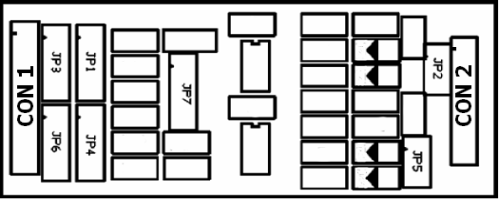
\includegraphics[width=0.50\textwidth,bb=0 0 500 200]{images/105.png}
	\caption{[FLEX105] Details of FLEX Multibus RS422 Module}
	\label{fig:105detail}
\end{figure}

\begin{small}
\begin{table}[!ht]
\centering
\begin{tabular}{|c|c|c|}
	\hline
	{\bf Jumper} & {\bf pos. 1-2} & {\bf pos. 2-3}\\
	\hline
	JP1 & TXEN\_dsPIC & TXEN +5V\\
	\hline
  JP2 & LOOPBACK\_0 & -\\
	\hline
  JP3 & TXEN\_dsPIC & TXEN GND\\
	\hline
  JP4 & TXEN\_dsPIC & TXEN +5V\\
	\hline
  JP5 & LOOPBACK\_1 & -\\
	\hline
  JP6 & TXEN\_dsPIC & TXEN GND\\
	\hline
  JP7 & RX\_0 & RX\_1\\
	\hline
  \multicolumn{3}{l}{\begin{tiny}Note: Default jumper settings are indicated by a $\bullet$\end{tiny}}\\
\end{tabular}
\caption{FLEX105 - Jumpers}
\label{tbl:105jps}
\end{table}
\end{small}

\begin{small}
\begin{table}[!ht]
\centering
\begin{tabular}{|c|l|}
	\hline
	Pin 1 & +5V\\
	\hline
  Pin 2 & TX\\
	\hline
  Pin 3 & TXEN\\
	\hline
  Pin 4 & RX\\
	\hline
  Pin 5 & -\\
	\hline
  Pin 6 & GND\\
	\hline
\end{tabular}
\caption{FLEX105 - CON1}
\label{tbl:105con1}
\end{table}
\end{small}

\begin{small}
\begin{table}[!ht]
\centering
\begin{tabular}{|c|l|}
	\hline
	Pin 1 & RS485+\_0\\
	\hline
  Pin 2 & RS485-\_0\\
	\hline
  Pin 3 & RS485+\_1\\
	\hline
  Pin 4 & RS485-\_1\\
	\hline
  Pin 5 & GND\\
	\hline
\end{tabular}
\caption{FLEX105 - CON2}
\label{tbl:105con2}
\end{table}
\end{small}



%+-+-+-+-+-+-+-+-+-+-+-+-+-+-+-+-+-+-+-+-+-+-+-+-+-+-+-+-+-+-+-+-+
\clearpage
\subsection{[FLEX106] FLEX Multibus CAN Module}
\label{subsec:106}
%+-+-+-+-+-+-+-+-+-+-+-+-+-+-+-+-+-+-+-+-+-+-+-+-+-+-+-+-+-+-+-+-+
The board, depicted in Figure ~\ref{fig:106}, is the CAN Module. It fits on slot 3 and/or slot 4 of the FLEX Multibus Base Daughter Board, refer Figure ~\ref{fig:101detail}.\\
\noindent The module can be used to export the CAN peripheral pins which are available on the dsPIC� using a CAN transceiver.\\

\begin{figure}[!ht]
	\centering
		\includegraphics[width=0.50\textwidth,bb=0 0 500 200]{images/flex106.jpg}
	\caption{[FLEX106] FLEX Multibus CAN Module}
	\label{fig:106}
\end{figure}


%^^^^^^^^^^^^^^^^^^^^^^^^^^^^^^^^^^^^^^^^^^^^^^^^^^
\subsubsection{Technical details}
\label{subsubsec:106tech}
%^^^^^^^^^^^^^^^^^^^^^^^^^^^^^^^^^^^^^^^^^^^^^^^^^^
\begin{figure}[!ht]
	\centering
		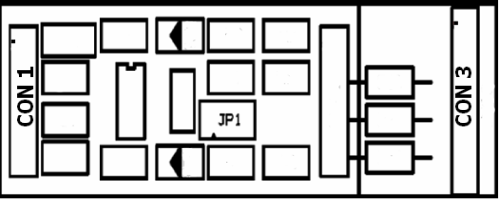
\includegraphics[width=0.50\textwidth,bb=0 0 500 200]{images/106.png}
	\caption{[FLEX106] Details of FLEX Multibus CAN Module}
	\label{fig:106detail}
\end{figure}

\begin{small}
\begin{table}[!ht]
\centering
\begin{tabular}{|c|c|c|}
	\hline
	{\bf Jumper} & {\bf pos. 1-2} & {\bf pos. 2-3}\\
	\hline
	JP1 & LOOPBACK & -\\
	\hline
  \multicolumn{3}{l}{\begin{tiny}Note: Default jumper settings are indicated by a $\bullet$\end{tiny}}\\
\end{tabular}
\caption{FLEX106 - Jumpers}
\label{tbl:106jps}
\end{table}
\end{small}

\begin{small}
\begin{table}[!ht]
\centering
\begin{tabular}{|c|l|}
	\hline
	Pin 1 & +5V\\
	\hline
  Pin 2 & RX\_CAN\\
	\hline
  Pin 3 & TX\_CAN\\
	\hline
  Pin 4 & GND\\
	\hline
\end{tabular}
\caption{FLEX106 - CON1}
\label{tbl:106con1}
\end{table}
\end{small}

\begin{small}
\begin{table}[!ht]
\centering
\begin{tabular}{|c|l|}
	\hline
	Pin 1 & -\\
	\hline
  Pin 2 & CAN+\\
	\hline
  Pin 3 & CAN-\\
	\hline
  Pin 4 & -\\
	\hline
  Pin 5 & GND\\
	\hline
\end{tabular}
\caption{FLEX106 - CON3}
\label{tbl:106con3}
\end{table}
\end{small}



%+-+-+-+-+-+-+-+-+-+-+-+-+-+-+-+-+-+-+-+-+-+-+-+-+-+-+-+-+-+-+-+-+
\clearpage
\subsection{[FLEX107] FLEX Multibus SPI Module}
\label{subsec:107}
%+-+-+-+-+-+-+-+-+-+-+-+-+-+-+-+-+-+-+-+-+-+-+-+-+-+-+-+-+-+-+-+-+
The board, depicted in Figure ~\ref{fig:107}, is the SPI Module. It fits on slot 6 of the FLEX Multibus Base Daughter Board, refer Figure ~\ref{fig:101detail}.\\
\noindent The module can be used to export one of the SPI peripheral pins which are available on the dsPIC�. The module also has a set of components which are used to protect the microcontroller pins from input signals that are not compatible with the specifications.\\

\begin{figure}[!ht]
	\centering
		\includegraphics[width=0.50\textwidth,bb=0 0 500 200]{images/flex107.jpg}
	\caption{[FLEX107] FLEX Multibus SPI Module}
	\label{fig:107}
\end{figure}


%^^^^^^^^^^^^^^^^^^^^^^^^^^^^^^^^^^^^^^^^^^^^^^^^^^
\subsubsection{Technical details}
\label{subsubsec:107tech}
%^^^^^^^^^^^^^^^^^^^^^^^^^^^^^^^^^^^^^^^^^^^^^^^^^^
\begin{figure}[!ht]
	\centering
		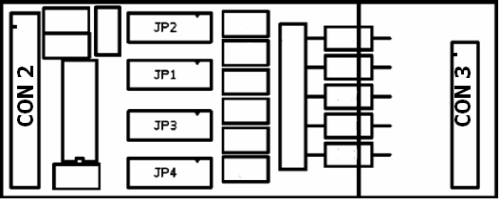
\includegraphics[width=0.50\textwidth,bb=0 0 500 200]{images/107.png}
	\caption{[FLEX107] Details of FLEX Multibus SPI Module}
	\label{fig:107detail}
\end{figure}

\begin{small}
\begin{table}[!ht]
\centering
\begin{tabular}{|c|c|c|}
	\hline
	{\bf Jumper} & {\bf pos. 1-2} & {\bf pos. 2-3}\\
	\hline
	JP1 & SPI\_DO & GND\\
	\hline
  JP2 & SPI\_CLK & GND\\
	\hline
  JP3 & SPI\_DO\_C & GND\\
	\hline
  JP4 & SPI\_SS & GND\\
	\hline
  \multicolumn{3}{l}{\begin{tiny}Note: Default jumper settings are indicated by a $\bullet$\end{tiny}}\\
\end{tabular}
\caption{FLEX107 - Jumpers}
\label{tbl:107jps}
\end{table}
\end{small}

\begin{small}
\begin{table}[!ht]
\centering
\begin{tabular}{|c|l|}
	\hline
	Pin 1 & +5V\\
	\hline
  Pin 2 & SPI\_DO\\
	\hline
  Pin 3 & SPI\_DI\\
	\hline
  Pin 4 & SPI\_CLK\\
	\hline
  Pin 5 & SPI\_SS\\
	\hline
  Pin 6 & GND\\
	\hline
\end{tabular}
\caption{FLEX107 - CON2}
\label{tbl:107con2}
\end{table}
\end{small}

\begin{small}
\begin{table}[!ht]
\centering
\begin{tabular}{|c|l|}
	\hline
	Pin 1 & SPI\_DO\_C\\
	\hline
  Pin 2 & SPI\_DI\_C\\
	\hline
  Pin 3 & SPI\_CLK\_C\\
	\hline
  Pin 4 & SPI\_SS\_C\\
	\hline
  Pin 5 & GND\\
	\hline
\end{tabular}
\caption{FLEX107 - CON3}
\label{tbl:107con3}
\end{table}
\end{small}



%+-+-+-+-+-+-+-+-+-+-+-+-+-+-+-+-+-+-+-+-+-+-+-+-+-+-+-+-+-+-+-+-+
\clearpage
\subsection{[FLEX108] FLEX Multibus Serial TTL Module}
\label{subsec:108}
%+-+-+-+-+-+-+-+-+-+-+-+-+-+-+-+-+-+-+-+-+-+-+-+-+-+-+-+-+-+-+-+-+
The board, depicted in Figure ~\ref{fig:108}, is the Serial TTL Module. It fits on slot 1 and/or slot 2 of the FLEX Multibus Base Daughter Board, refer Figure ~\ref{fig:101detail}.\\
\noindent This module can be used to export the UART pins linked to the UART peipherals on the dsPIC� by using signals which are compatible with TTL electronic equipments. The module also has a set of components which are used to protect the microcontroller pins from input signals which are not compatible with the specifications.\\

\begin{figure}[!ht]
	\centering
		\includegraphics[width=0.50\textwidth,bb=0 0 500 200]{images/flex108.jpg}
	\caption{[FLEX108] FLEX Multibus Serial TTL Module}
	\label{fig:108}
\end{figure}


%^^^^^^^^^^^^^^^^^^^^^^^^^^^^^^^^^^^^^^^^^^^^^^^^^^
\subsubsection{Technical details}
\label{subsubsec:108tech}
%^^^^^^^^^^^^^^^^^^^^^^^^^^^^^^^^^^^^^^^^^^^^^^^^^^
\begin{figure}[!ht]
	\centering
		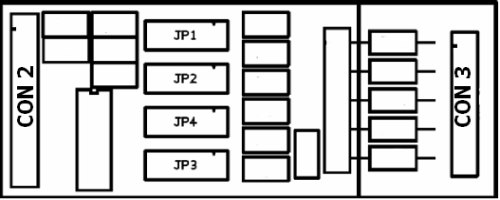
\includegraphics[width=0.50\textwidth,bb=0 0 500 200]{images/108.png}
	\caption{[FLEX108] Details of FLEX Multibus Serial TTL Module}
	\label{fig:108detail}
\end{figure}

\begin{small}
\begin{table}[!ht]
\centering
\begin{tabular}{|c|c|c|}
	\hline
	{\bf Jumper} & {\bf pos. 1-2} & {\bf pos. 2-3}\\
	\hline
	JP1 & TX\_1 & GND\\
	\hline
  JP2 & SCK\_1 & GND\\
	\hline
  JP3 & TX\_TTL & GND\\
	\hline
  JP4 & RTS\_TTL & GND\\
	\hline
  \multicolumn{3}{l}{\begin{tiny}Note: Default jumper settings are indicated by a $\bullet$\end{tiny}}\\
\end{tabular}
\caption{FLEX108 - Jumpers}
\label{tbl:108jps}
\end{table}
\end{small}

\begin{small}
\begin{table}[!ht]
\centering
\begin{tabular}{|c|l|}
	\hline
	Pin 1 & +5V\\
	\hline
  Pin 2 & TX\_1\\
	\hline
  Pin 3 & SCK\_1\\
	\hline
  Pin 4 & RX\_1\\
	\hline
  Pin 5 & FRCK\_1\\
	\hline
  Pin 6 & GND\\
	\hline
\end{tabular}
\caption{FLEX108 - CON2}
\label{tbl:108con2}
\end{table}
\end{small}

\begin{small}
\begin{table}[!ht]
\centering
\begin{tabular}{|c|l|}
	\hline
	Pin 1 & CTS\_TTL\\
	\hline
  Pin 2 & RX\_TTL\\
	\hline
  Pin 3 & TX\_TTL\\
	\hline
  Pin 4 & RTS\_TTL\\
	\hline
  Pin 5 & GND\\
	\hline
\end{tabular}
\caption{FLEX108 - CON3}
\label{tbl:108con3}
\end{table}
\end{small}
%|||||||||||||||||||||||||||||||||||||||||||||||||||||||||
%+-+-+-+-+-+-+-+-+-+-+-+-+-+-+-+-+-+-+-+-+-+-+-+-+-+-+-+-+-+-+-+-+
\clearpage
\subsection{Multibus I2C Module}
\label{subsec:i2c}
%+-+-+-+-+-+-+-+-+-+-+-+-+-+-+-+-+-+-+-+-+-+-+-+-+-+-+-+-+-+-+-+-+
The I2C Module fits on slot 5 of the FLEX Multibus Base Daughter Board, refer Figure ~\ref{fig:101detail}.\\
\noindent This module can be used to connect in a safe way an I2C bus to one of the I2C peripherals of the dsPIC�. The protection includes protection from spikes, as well as hot insertions and hot extractions.\\
%|||||||||||||||||||||||||||||||||||||||||||||||||||||||||




%+-+-+-+-+-+-+-+-+-+-+-+-+-+-+-+-+-+-+-+-+-+-+-+-+-+-+-+-+-+-+-+-+
\clearpage
\subsection{[FLEX109] FLEX Demo Daughter Board}
\label{subsec:109}
%+-+-+-+-+-+-+-+-+-+-+-+-+-+-+-+-+-+-+-+-+-+-+-+-+-+-+-+-+-+-+-+-+
The FLEX Demo Board, as depicted in Figures ~\ref{fig:109a} and ~\ref{fig:109b}, is a FLEX Daughter Board, refer Section ~\ref{sec:daughter}, targeted specifically for educational institutions e.g. Schools and Universities.\\

\begin{figure}[!ht]
	\centering
		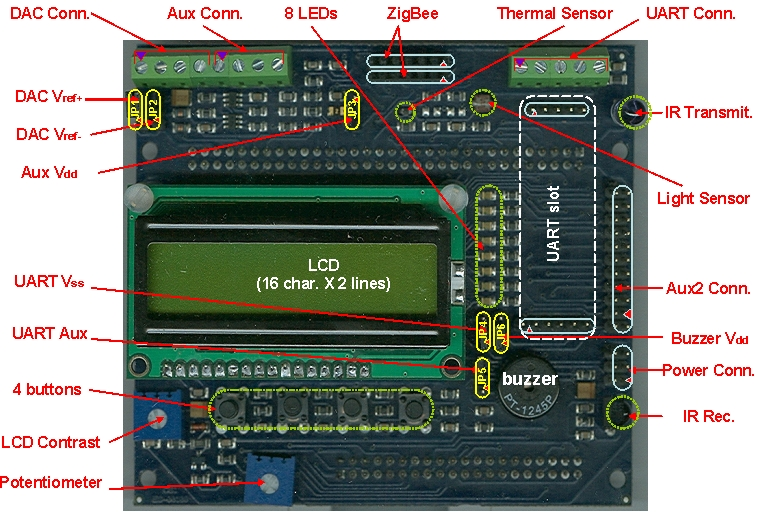
\includegraphics[width=0.90\textwidth,bb=0 0 758 512]{images/flex109a.jpg}
	\caption{[FLEX109] FLEX Demo Daughter Board - front side}
	\label{fig:109a}
\end{figure}
\begin{figure}[!ht]
	\centering
		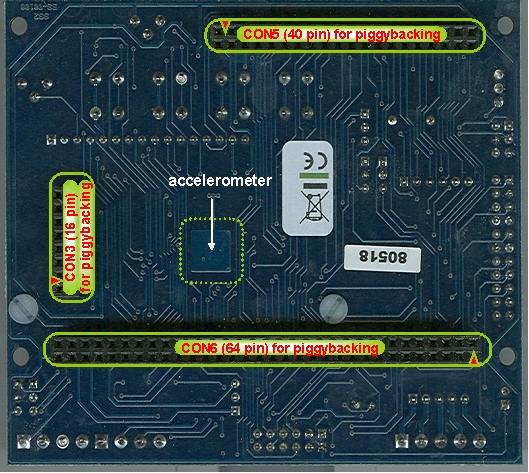
\includegraphics[width=0.90\textwidth,bb=0 0 529 473]{images/flex109b.jpg}
	\caption{[FLEX109] FLEX Demo Daughter Board - back side}
	\label{fig:109b}
\end{figure}

\noindent The FLEX Demo Board fits directly on FLEX Base Boards (FLEX Full, refer Subsection ~\ref{subsec:001}/FLEX Light, refer Subsection ~\ref{subsec:003}) and it adds-on a lot of most commonly used features that are used for carrying out prototyping and laboratory experiments.\\

\noindent The features hosted on Demo Board are:
\begin{itemize}
  \item 2 DAC outputs (12 bit resolution)
  \item 3-axis accelerometer (selectable range from 1.5g to 6g)
  \item Direct support for quadrature encoder
  \item Set of 4 Push buttons
  \item Set of 8 LEDs
  \item LCD (16 characters x 2 lines)
  \item Buzzer
  \item Potentiometer
  \item Thermal sensor
  \item Light sensor
  \item InfraRed receiver and transmitter
  \item ZigBee connector
  \item Socket for Multibus serial modules (one of FLEX103, FLEX104, FLEX105, and FLEX108)
  \item USB wiring for FLEX Full Base Board
\end{itemize}

\noindent {\tt Note: The FLEX Demo Board is fully supported by Scilab/Scicos code generator, where specific blocks are available to directly control the main peripherals. Hence, applications can be entirely generated without writing any C code!}\\


%^^^^^^^^^^^^^^^^^^^^^^^^^^^^^^^^^^^^^^^^^^^^^^^^^^
\subsubsection{Technical details}
\label{subsubsec:109tech}
%^^^^^^^^^^^^^^^^^^^^^^^^^^^^^^^^^^^^^^^^^^^^^^^^^^
\begin{figure}[!ht]
	\centering
		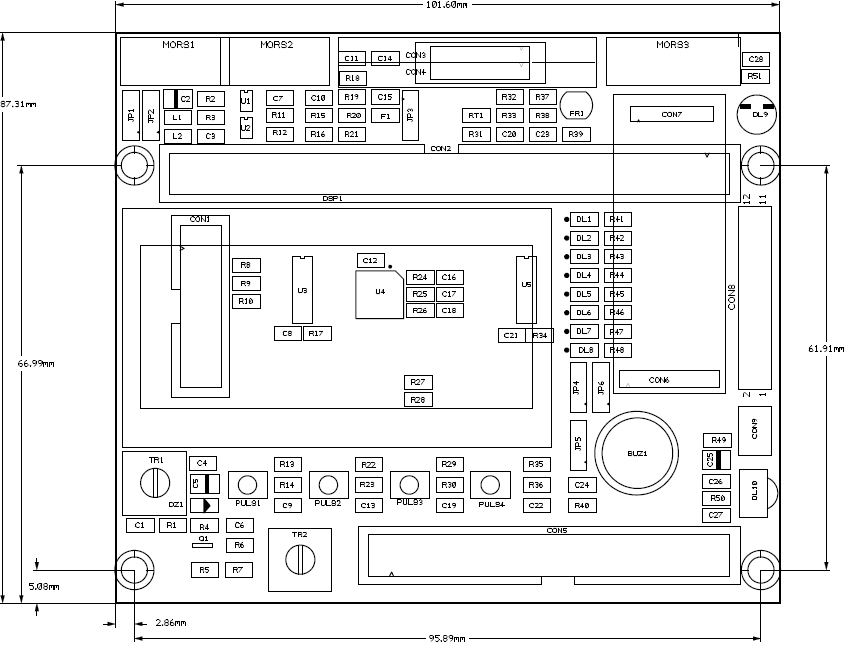
\includegraphics[width=0.90\textwidth,bb=0 0 845 645]{images/109mec.png}
	\caption{[FLEX109] Dimensions of FLEX Demo Daughter Board}
	\label{fig:109mec}
\end{figure}
\begin{figure}[!ht]
	\centering
		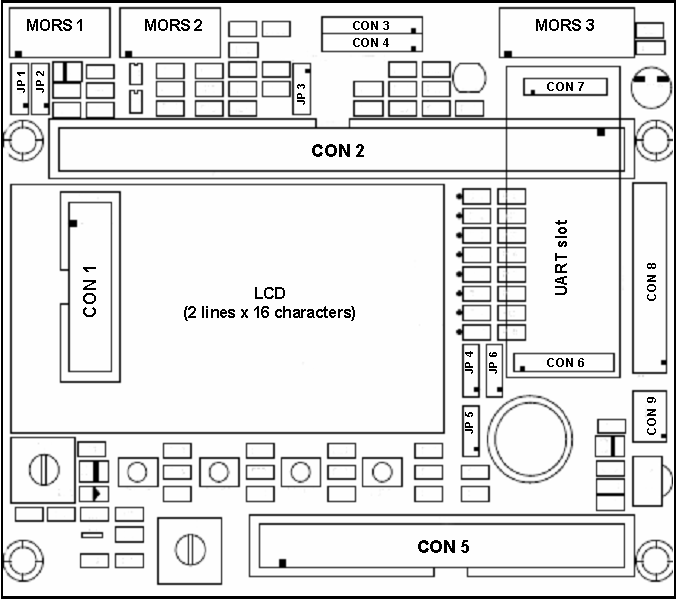
\includegraphics[width=0.90\textwidth,bb=0 0 677 599]{images/109.png}
	\caption{[FLEX109] Details of FLEX Demo Daughter Board}
	\label{fig:109detail}
\end{figure}

\begin{small}
\begin{table}[!ht]
\centering
\begin{tabular}{|c|l|}
  \hline
  Pin 1 & Analog Output 1\\
	\hline
	Pin 2 & GND \\
	\hline
	Pin 3 & Analog Output 2\\
	\hline
	Pin 4 & GND \\
	\hline
\end{tabular}
\caption{FLEX109 - MORS1 (DAC Connector)}
\label{tbl:109mors1}
\end{table}
\end{small}

\begin{small}
\begin{table}[!ht]
\centering
\begin{tabular}{|c|l|}
  \hline
	Pin 1 & Data 1\\
	\hline
	Pin 2 & Data 2\\
	\hline
	Pin 3 & Vout/+5V (selectable)\\
	\hline
	Pin 4 & GND\\
	\hline
\end{tabular}
\caption{FLEX109 - MORS2 (AUX Connector)}
\label{tbl:109mors2}
\end{table}
\end{small}

\begin{small}
\begin{table}[!ht]
\centering
\begin{tabular}{|c|l|}
  \hline
	Pin 1 & CTS (232/TTL)/TX+ (422)\\
	\hline
	Pin 2 & RX (232/TTL)/TX- (422)/485- (485)\\
	\hline
	Pin 3 & TX (232/TTL)/RX+ (422)/485+ (485)\\
	\hline
	Pin 4 & RTS (232/TTL)/RX- (422)\\
	\hline
	Pin 5 & GND\\
	\hline
\end{tabular}
\caption{FLEX109 - MORS3 (UART Connector)}
\label{tbl:109mors3}
\end{table}
\end{small}

\begin{small}
\begin{table}[!ht]
\centering
\begin{tabular}{|l|l|}
  \hline
	DL1 (yellow) & RF0\\
	\hline
	DL2 (yellow) & RF1\\
	\hline
	DL3 (yellow) & RF2\\
	\hline
	DL4 (yellow) & RF3\\
	\hline
	DL5 (yellow) & RD8\\
	\hline
	DL6 (yellow) & RD9\\
	\hline
	DL7 (yellow) & RD10\\
	\hline
	DL8 (yellow) & RD11\\
	\hline
\end{tabular}
\caption{FLEX109 - LEDs}
\label{tbl:109leds}
\end{table}
\end{small}


\begin{small}
\begin{table}[!ht]
\centering
\begin{tabular}{|l|c|c|}
  \hline
  {\bf Jumper} & {\bf pos. 1-2} & {\bf pos. 2-3}\\
  \hline
	[JP1] DAC Vref+ & $\bullet$ +5V & +3.3V\\
	\hline
	[JP2] DAC Vref- & $\bullet$ GND & GNDout\\
	\hline
	[JP3] Aux Vdd & $\bullet$ Vout & +5V\\
	\hline
	[JP4] UART Vss & $\bullet$ GND & GNDout\\
	\hline
	[JP5] UART Aux & INT (Konnex/EIB) & $\bullet$ RTS (232/422/TTL)\\
	\hline
	[JP6] Buzzer Vdd & $\bullet$ Vout & +5V\\
	\hline
  \multicolumn{3}{l}{\begin{tiny}Note: Default jumper settings are indicated by a $\bullet$\end{tiny}}\\
\end{tabular}
\caption{FLEX109 - Jumpers}
\label{tbl:109jps}
\end{table}
\end{small}

\begin{small}
\begin{table}[!ht]
\centering
\begin{tabular}{|c|c|c|c|}
  \hline
	{\bf Push Btn.} & {\bf pin} & {\bf pos. 1-2 (normal)} & {\bf pos. 2-3 (pressed)}\\
	\hline
	PULS1 & RD4 & +5V & GND\\
	\hline
	PULS2 & RD5 & +5V & GND\\
	\hline
	PULS3 & RD6 & +5V & GND\\
	\hline
	PULS4 & RD15 & +5V & GND\\
	\hline
\end{tabular}
\caption{FLEX109 - Push Buttons}
\label{tbl:109btns}
\end{table}
\end{small}

\begin{small}
\begin{table}[!ht]
\centering
\begin{tabular}{|l|l||l|l|}
  \hline
	\multicolumn{2}{|c||}{\bf CON3} & \multicolumn{2}{c|}{\bf CON4}\\
	\hline
	Pin 1 & +3.3V & Pin 1 & GND\\
	\hline
	Pin 2 & Reset & Pin 2 & Vreg\\
	\hline
	Pin 3 & FIFO & Pin 3 & CSN\\
	\hline
	Pin 4 & SDO & Pin 4 & SDI\\
	\hline
	Pin 5 & SCK & Pin 5 & CCA\\
	\hline
	Pin 6 & SFD & Pin 6 & FIFOP\\
	\hline
\end{tabular}
\caption{FLEX109 - CON3+CON4 (ZigBee Connector)}
\label{tbl:109con3con4}
\end{table}
\end{small}

\begin{small}
\begin{table}[!ht]
\centering
\begin{tabular}{|c|l|}
	\hline
	Pin 1 & +5V\\
	\hline
	Pin 2 & RF5 (TX1)\\
	\hline
	Pin 3 & RF12 (SCK1)\\
	\hline
	Pin 4 & RF4 (RX1)\\
	\hline
	Pin 5 & JP6 (default pos. 1-2 i.e. Vout)\\
	\hline
	Pin 6 & JP4 (default pos. 2.3 i.e. GND)\\
	\hline
\end{tabular}
\caption{FLEX109 - CON6 (Connected to Serial TTL)}
\label{tbl:109con6}
\end{table}
\end{small}

\begin{small}
\begin{table}[!ht]
\centering
\begin{tabular}{|c|l|}
	\hline
	Pin 1 & CTS (232/TTL)/TX+ (422)\\
	\hline
	Pin 2 & RX (232/TTL)/TX- (422)/485- (485)\\
	\hline
	Pin 3 & TX (232/TTL)/RX+ (422)/485+ (485)\\
	\hline
	Pin 4 & RTS (232/TTL)/RX- (422)\\
	\hline
	Pin 5 & GND\\
	\hline
\end{tabular}
\caption{FLEX109 - CON7 (connected to MORS3)}
\label{tbl:109con7}
\end{table}
\end{small}

\begin{small}
\begin{table}[!ht]
\centering
\begin{tabular}{|l|l||l|l|}
	\hline
	Pin 1 & Encoder Index & Pin 2 & PWMout 1L\\
	\hline
	Pin 3 & Encoder Channel A & Pin 4 & PWMout 1H\\
	\hline
	Pin 5 & Encoder Channel B & Pin 6 & PWMout 2L\\
	\hline
	Pin 7 & OC8 & Pin 8 & PWMout 2H\\
	\hline
	Pin 9 & Analog Input 19 & Pin 10 & PWMout 3L\\
	\hline
	Pin 11 & OC3 & Pin 12 & PWMout 3H\\
	\hline
	Pin 13 & DSPPCLK & Pin 14 & PWMout 4L\\
	\hline
	Pin 15 & DSPPDATA & Pin 16 & PWMout 4H\\
	\hline
	Pin 17 & DSPMCLR & Pin 18 & Analog Input 20\\
	\hline
	Pin 19 & AV SSext & Pin 20 & Analog Input 21\\
	\hline
	Pin 21 & AV DDext & Pin 22 & GND\\
	\hline
\end{tabular}
\caption{FLEX109 - CON8 (AUX2 Connector)}
\label{tb1:109con8}
\end{table}
\end{small}

\begin{small}
\begin{table}[!ht]
\centering
\begin{tabular}{|c|l|}
	\hline
	Pin 1 & Vout\\
	\hline
	Pin 2 & GNDout\\
	\hline
	Pin 3 & +5V\\
	\hline
	Pin 4 & GND\\
	\hline
	Pin 5 & +3.3V\\
	\hline
	Pin 6 & GND\\
	\hline
\end{tabular}
\caption{FLEX109 - CON9 (Power Connector)}
\label{tbl:109con9}
\end{table}
\end{small}
%-----------------------------------------------------------------
\section{Packs}
\label{sec:packs}
%-----------------------------------------------------------------

%+-+-+-+-+-+-+-+-+-+-+-+-+-+-+-+-+-+-+-+-+-+-+-+-+-+-+-+-+-+-+-+-+
\subsection{[FLEX110] FLEX multibus pack}
\label{subsec:110}
%+-+-+-+-+-+-+-+-+-+-+-+-+-+-+-+-+-+-+-+-+-+-+-+-+-+-+-+-+-+-+-+-+
The FLEX multibus pack, depicted in the Figure ~\ref{fig:flex110}, with most widely used serial communication standards is now available!\\

\begin{figure}[!ht]
	\centering
		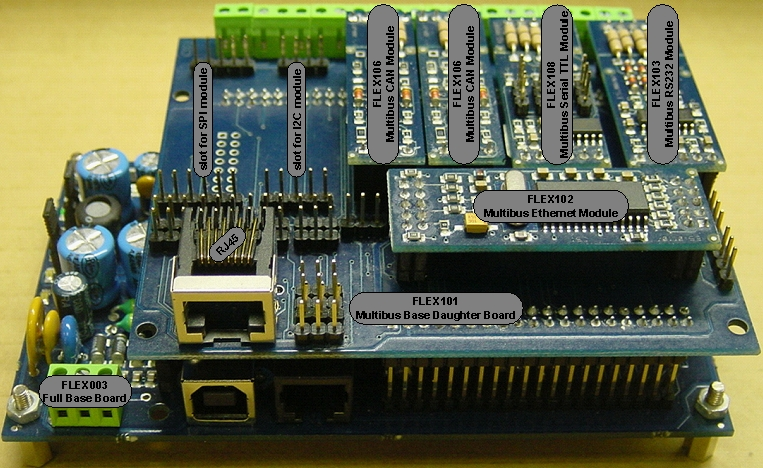
\includegraphics[width=0.90\textwidth, bb=0 0 763 468]{images/flex110.jpg}
	\caption{[FLEX110] FLEX multibus pack}
	\label{fig:flex110}
\end{figure}

\noindent The FLEX Multibus Base Daughter Board is piggybacked on FLEX Base Boards (FLEX Full, refer Subsection ~\ref{subsec:001}/FLEX Light refer Subsection ~\ref{subsec:003}) and in turn, the FLEX Multibus modules are piggybacked on the FLEX Multibus Base Daughter Board.\\

\noindent The FLEX multibus pack consists of:
\begin{itemize}
  \item 1 x [FLEX101] FLEX Multibus Base Daughter Board (bare board without Ethernet port), refer Subsection ~\ref{subsec:101}
  \item 1 x [FLEX102] FLEX Multibus Ethernet Module + 1 x RJ45 Ethernet port (to be soldered), refer Subsection ~\ref{subsec:102}
  \item 2 x [FLEX103] FLEX Multibus RS232 Modules, refer Subsection ~\ref{subsec:103}
  \item 1 x [FLEX104] FLEX Multibus RS485 Module, refer Subsection ~\ref{subsec:104}
  \item 1 x [FLEX105] FLEX Multibus RS422 Module, refer Subsection ~\ref{subsec:105}
  \item 2 x [FLEX106] FLEX Multibus CAN Modules, refer Subsection ~\ref{subsec:106}
  \item 1 x [FLEX107] FLEX Multibus SPI Module, refer Subsection ~\ref{subsec:107}
  \item 1 x [FLEX108] FLEX Multibus Serial TTL Module, refer Subsection ~\ref{subsec:108}
\end{itemize}

{\tt Note: The FLEX multibus pack does not include FLEX Base Board.}\\


%^^^^^^^^^^^^^^^^^^^^^^^^^^^^^^^^^^^^^^^^^^^^^^^^^^
\subsubsection{Technical details}
\label{subsubsec:110tech}
%^^^^^^^^^^^^^^^^^^^^^^^^^^^^^^^^^^^^^^^^^^^^^^^^^^
Refer technical details of:\\
\indent $\bullet$ \hspace{0.1cm} [FLEX101] FLEX Multibus Base Daughter Board, refer Sub-subsection ~\ref{subsubsec:101tech}\\
\indent $\bullet$ \hspace{0.1cm} [FLEX102] FLEX Multibus Ethernet Module, refer Sub-subsection ~\ref{subsubsec:102tech}\\
\indent $\bullet$ \hspace{0.1cm} [FLEX103] FLEX Multibus RS232 Module, refer Sub-subsection ~\ref{subsubsec:103tech}\\
\indent $\bullet$ \hspace{0.1cm} [FLEX104] FLEX Multibus RS485 Module, refer Sub-subsection ~\ref{subsubsec:104tech}\\
\indent $\bullet$ \hspace{0.1cm} [FLEX105] FLEX Multibus RS422 Module, refer Sub-subsection ~\ref{subsubsec:105tech}\\
\indent $\bullet$ \hspace{0.1cm} [FLEX106] FLEX Multibus CAN Modules, refer Sub-subsection ~\ref{subsubsec:106tech}\\
\indent $\bullet$ \hspace{0.1cm} [FLEX107] FLEX Multibus SPI Module, refer Sub-subsection ~\ref{subsubsec:107tech}\\
\indent $\bullet$ \hspace{0.1cm} [FLEX108] FLEX Multibus Serial TTL Module, refer Sub-subsection ~\ref{subsubsec:108tech}\\




%+-+-+-+-+-+-+-+-+-+-+-+-+-+-+-+-+-+-+-+-+-+-+-+-+-+-+-+-+-+-+-+-+
\clearpage
\subsection{[FLEX111] FLEX fast track suite}
\label{subsec:111}
%+-+-+-+-+-+-+-+-+-+-+-+-+-+-+-+-+-+-+-+-+-+-+-+-+-+-+-+-+-+-+-+-+
FLEX boards enable easy and fast development of embedded applications for the Microchip dsPIC� DSC micro-controller. The easily expandable hardware, combined with widely available software applications, makes FLEX ideal for Schools and Universities for fast track education.\\

\begin{figure}[!ht]
	\centering
		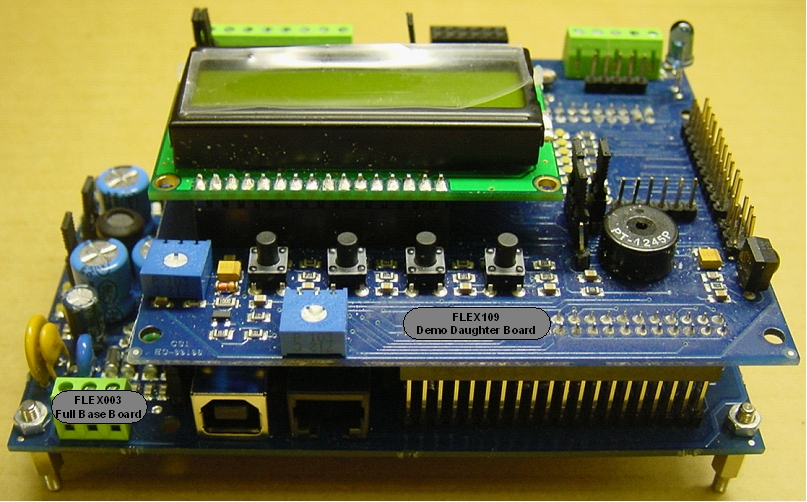
\includegraphics[width=0.90\textwidth, bb=0 0 807 502]{images/flex111.jpg}
	\caption{[FLEX111] FLEX fast track suite}
	\label{fig:flex111}
\end{figure}

\noindent As depicted in the Figure ~\ref{fig:flex111}, the FLEX Demo Daughter Board is one of the few educational boards offering 2 DAC outputs, a 3-axis accelerometer, and a direct support for an encoder. Moreover, with the direct support of the Scilab code generator, applications can be entirely generated without writing any C code.\\

\noindent The FLEX fast track suite consists of:
\begin{itemize}
  \item Hardware
    \begin{itemize}
      \item 1 x [FLEX003] FLEX Full Base Board, refer Subsection ~\ref{subsec:003}
      \item 1 x [FLEX109] FLEX Demo Daughter Board, refer Subsection ~\ref{subsec:109}
    \end{itemize}
  \item Free Software
    \begin{itemize}
      \item ERIKA Enterprise real-time kernel
      \item Scilab/Scicos simulation and code generation tool
    \end{itemize}
  \item Support (available on the web-site)
    \begin{itemize}
      \item Ready to run demos with source code
      \item Application notes
      \item User Forums
      \item Wiki
    \end{itemize}
\end{itemize}


%^^^^^^^^^^^^^^^^^^^^^^^^^^^^^^^^^^^^^^^^^^^^^^^^^^
\subsubsection{Technical details}
\label{subsubsec:111tech}
%^^^^^^^^^^^^^^^^^^^^^^^^^^^^^^^^^^^^^^^^^^^^^^^^^^
Refer technical details of:\\
\indent $\bullet$ \hspace{0.1cm} [FLEX003] FLEX Full Base Board, refer Sub-subsection ~\ref{subsubsec:003tech}\\
\indent $\bullet$ \hspace{0.1cm} [FLEX109] FLEX Demo Daughter Board, refer Sub-subsection ~\ref{subsubsec:109tech}\\
%-----------------------------------------------------------------
\section{Hardware Customisation}
\label{sec:custom}
%-----------------------------------------------------------------

A number of possible extensions can be made to the FLEX Base Boards, refer Section ~\ref{sec:base}, to add new functionalities, sensors, network connections, actuators, etc. Simple extensions can be made by hand by either using a Thru Hole Board, refer Subsection ~\ref{subsec:100}, or using a Multibus Base Board, refer Subsection ~\ref{subsec:101}. More decent extensions may require some expertise. This may require some special equipment (e.g. mounting SMD components) to implement a fully functional board. To avoid these problems, Embedded Solutions Srl can handle you specific needs and create a customised Daughter Board for FLEX, refer Section ~\ref{sec:daughter}.\\

\noindent Depending on the number of items to be produced, it could be convenient to re-engineer an entire board together with the Base and the Daughter Boards to save on size, weight, and power consumption. Embedded Solutions also handles prototyping of multilayer boards with SMT and PTH technologies.\\ \\

\noindent {\tt Contact us for customised FLEX Daughter Boards!}\\
%=================================================================
\chapter{Software for \flex}
\label{ch:software}
%=================================================================
%\chapter{Sofware development for the \flex\ boards}
%\label{ch:ee-flex}
The \flex\ boards comes with a rich software infrastructure which symplifies the appli-
cation development.

\section{\ee}
First of all, \flex\ comes with \ee\ as the default software
development environment. In particular, \ee\ for Microchip dsPIC (R)
DSC micro-controller family is a complete open-source\footnote{\ee\ is
distributed under the GPL+Linking exception license} RTOS implementing
the OS, OIL, and ORTI part of the OSEK/VDX standard
(\url{http://www.osek-vdx.org}). \ee\ includes the state of the art
real- time technology as well as the \rtd\ configuration tool, which
allows easy design and optimization of a real-time application.

\section{Libraries for \flex}
\ee\ fully supports the \flex\ boards and all the
Daughter Boards. A complete set of libraries allows the exploitation
of all the features provided. The development of complex applications
based on the \flex\ Base Board and available Daughter Boards is
simplified by a well documented and clear set of primitives.  The
needed libraries can be configured using the \rtd\ tool, letting the
developer to dedicate the efforts to the implementation of the program
logic.

\section{Template applications}
A set of template applications using the \flex\ boards are also
available. These applica- tions can be instantiated as \rtd\ projects
by selecting the appropriate template at project creation time.

\section{Scilab and Scicos code generator}
Finally, a code generator for Scilab and Scicos designs is also
available. The code generator has been developed in collaboration
with Simone Mannori from INRIA (FR), and Roberto Bucher from SUPSI
Lugano. 

Please check the Evidence web site
\url{http://www.evidence.eu.com} to get updated documentation and
manuals about the Scilab/Scicos code generator support.

%=================================================================
\chapter{FLEX Producers and Distributors}
\label{ch:prod_dist}
%=================================================================

%-----------------------------------------------------------------
\section{FLEX Producers}
\label{sec:producers}
%-----------------------------------------------------------------
\begin{tabular}{p{0.45\columnwidth} p{0.45\columnwidth}}
  
\includegraphics[width=0.25\textwidth, bb=0 0 417 194]{../common/LogoEvidence.png}
  &
  
\includegraphics[width=0.25\textwidth, bb=0 0 115 66]{../common/LogoES.png}\\
  \\
\end{tabular}

\noindent The FLEX platform is a result of  synergistic effort of two Italian companies working in the field of embedded systems: Evidence Srl and Embedded Solutions. These two companies combined their respective skills on real-time systems and electronic boards development, to create this complete, easy-to-use, compact solution for creating complex applications based on the Microchip dsPIC� DSC micro-controller.\\

\noindent In particular, 
\begin{itemize}
\item Evidence Srl provided a GPL version of the Erika Enterprise RTOS, including template applications for the FLEX Boards.
\item Embedded Solutions Srl provided the hardware design and is also the producer of the FLEX hardware.
\end{itemize}

\noindent In addition to the availability of a set of Daughter Boards, it is also possible to make customised Daughter Boards. If you are interested in having customised FLEX hardware, please check Section ~\ref{sec:custom}.\\


\pagebreak
%-----------------------------------------------------------------
\section{FLEX Distributors}
\label{sec:distributors}
%-----------------------------------------------------------------
FLEX Boards are only sold though dristributors.\\
{\tt Please refer the distributors list, Table ~\ref{tbl:d_list}, to buy FLEX Boards!}\\

%+-+-+-+-+-+-+-+-+-+-+-+-+-+-+-+-+-+-+-+-+-+-+-+-+-+-+-+-+-+-+-+-+
\subsection{Where is FLEX available?}
\label{subsec:dist}
%+-+-+-+-+-+-+-+-+-+-+-+-+-+-+-+-+-+-+-+-+-+-+-+-+-+-+-+-+-+-+-+-+
\begin{small}
\begin{table} [ht]
\centering
  \begin{tabular}{|l p{0.6\columnwidth}|}
    \hline
    {\bf Location} & {\bf Distributor}\\
    \hline
    {\bf {\em Europe:}} & \\
    Italy & EMCElettronica\newline \url{http://dev.emcelettronica.com/}\\
    Italy & InWare srl\newline \url{http://www.elettroshop.it/}\\
    France & M.N.I.S.\newline \url{http://www.mnis.fr/}\\
    UK & Farnell\newline \url{http://www.farnell.co.uk/}\\
    
    {\bf {\em Asia:}} & \\
    Japan & IPIShop\newline \url{http://www.ipishop.com/}\\
    
    {\bf {\em USA:}} & \\
    USA & Microcontroller Shop\newline \url{http://microcontrollershop.com/}\\
    USA & Spark Fun Electronics Inc.\newline \url{http://www.sparkfun.com/}\\
    
    {\bf {\em South America:}} & \\
    Chile \& South America & Ingenier�a MCI Ltda. (Olimex Chile)\newline \url{http://www.olimex.cl/}\\
    
    {\bf {\em Worldwide:}} & \\
    Worldwide & Farnell\newline \url{http://www.farnell.com/}\\
    Worldwide & Microchip Direct\newline \url{http://www.microchipdirect.com/}\\
    \hline
  \end{tabular}
\caption{FLEX Distributors}
\label{tbl:d_list}
\end{table}
\end{small}

%+-+-+-+-+-+-+-+-+-+-+-+-+-+-+-+-+-+-+-+-+-+-+-+-+-+-+-+-+-+-+-+-+
\subsection{What if my country is not listed?}
\label{subsec:no_dist}
%+-+-+-+-+-+-+-+-+-+-+-+-+-+-+-+-+-+-+-+-+-+-+-+-+-+-+-+-+-+-+-+-+
Please select the nearest distributor to your site!\\


%+-+-+-+-+-+-+-+-+-+-+-+-+-+-+-+-+-+-+-+-+-+-+-+-+-+-+-+-+-+-+-+-+
\subsection{Would you like to become a distributor?}
\label{subsec:new_dist}
%+-+-+-+-+-+-+-+-+-+-+-+-+-+-+-+-+-+-+-+-+-+-+-+-+-+-+-+-+-+-+-+-+
If you are a distributor and you want to distribute FLEX Boards in selected countries, please do not hesitate to contact us!\\


%\bibliographystyle{plain}
%\bibliography{../common/biblio}
\printindex
\end{document}
